\documentclass[11pt]{article}
\usepackage[utf8]{inputenc} 
\usepackage[T1]{fontenc} 	% Font encoding
\usepackage{amsmath} 		% Math package
\usepackage{mathtools} 		% Adds the declare paired 
							% delimeter command to make costom \abs and \norm
\usepackage{breqn}		 	% Adds dmath environment for automated brakeline
\usepackage{xfrac}			% Adds slanted fractions (sfrac)
\usepackage{cancel}			% Adds the cancel command, a slash through the symbol(s)
\usepackage{tabularx}		% Adds adjustable width on tabulars
\usepackage{tabu}           % colored font in tabular
\usepackage{cuted}			% Adds the strip command, pagewidth text in a twocolumn
							% environment.  
\usepackage{hyperref}
\usepackage{siunitx}		% SI-enheter
\usepackage{tablefootnote}
\usepackage{times}
\usepackage{listings}
\usepackage{parskip}
\usepackage[dvipsnames]{xcolor,colortbl} % expanded colors and table colors

% Capitalized headings
\usepackage{sectsty}

% Set margins
\usepackage[a4paper, margin=0.75in]{geometry}

% Alghorithm packages:
\usepackage{algorithm}
\usepackage[noend]{algpseudocode}

% colored box
\usepackage[most]{tcolorbox}

% Numbers within section
\numberwithin{equation}{section}
\numberwithin{figure}{section}

% Start custom \abs \norm 
\DeclarePairedDelimiter\abs{\lvert}{\rvert}%
\DeclarePairedDelimiter\norm{\lVert}{\rVert}%

\newcommand{\equ}[1]{{\small\begin{align*}#1\end{align*}}}
\newcommand{\mc}[1]{\mathcal{#1}}
\newcommand{\ita}[1]{\textit{#1}}
\newcommand{\ma}[1]{$#1$}
\newcommand{\eq}[1]{{\small\begin{align}#1\end{align}}}
\newcommand{\mat}[1]{\begin{matrix}#1\end{matrix}}
\renewcommand\vec[1]{\mathbf{#1}}
\renewcommand\vec[1]{\mathbf{#1}}
\renewcommand\vec[1]{\mathbf{#1}}
\newcommand{\OP}[1]{\mathbf{\widehat{#1}}}
\newcommand{\op}[1]{\hat{#1}}
\newcommand{\unit}[1]{\mathbf{\hat{#1}}}

%% Invisible subsection
\newcommand\invisiblesubsection[1]{%
  \refstepcounter{subsection}%
  \addcontentsline{toc}{subsection}{\protect\numberline{\thesubsection}#1}%
  \subsectionmark{#1}}


%% Section renewcomands
\renewcommand{\thesection}{\Alph{section}.}
\renewcommand{\thesubsection}{\arabic{subsection}.}
\renewcommand{\thesubsubsection}{\arabic{subsection}.\arabic{subsubsection}}
\renewcommand{\theequation}{\arabic{subsection}.\arabic{equation}}
\renewcommand{\thefigure}{\arabic{subsection}.\arabic{figure}}




\title{Exam Notes---FYS4460}
\author{Alexander Fleischer}




\begin{document}

\maketitle



\sectionfont{\centering\MakeUppercase}

\tcbset{enhanced, width=\textwidth, left=40pt,
    colback=black!5!white,
    boxrule=0.4pt,
    colframe=white!40!black,sharp corners,fonttitle=\bfseries,
    rounded corners=southeast,arc is angular,arc=3mm,
    underlay={%
    \path[fill=tcbcol@back!80!black]
        ([yshift=3mm]interior.south east)--++ (-0.4,-0.1)--++ (0.1,-0.2);
    \path[draw=tcbcol@frame,shorten <=-0.05mm,shorten >=-0.05mm] 
        ([yshift=3mm]interior.south east)--++ (-0.4,-0.1)--++ (0.1,-0.2);
    \path[fill=white!40!black,draw=none] (interior.south west) 
        rectangle node[white]{\Huge\bfseries \thesubsection} 
        ([xshift=40pt]interior.north west);
    }, drop fuzzy shadow}

\tableofcontents
\newpage

\section{Molecular Dynamics}

\setcounter{subsubsection}{0}
\invisiblesubsection{Molecular-dynamics algorithms}
\begin{tcolorbox}[title=Molecular-dynamics algorithms]
    Discuss the algorithms for molecular-dynamics modeling:
    Potentials, integration, cut-off, periodic boundary conditions,
    efficiency improvements.
\end{tcolorbox}

\subsubsection{Potentials} 
The potentials describe the interactions between
objects through $\vec F = -\vec\nabla U$.
Two particles may interact on each other, two-body interactions,
which is the simplest potential. If three or more
particles interact on each other, we have a many-body interaction.

In MD, we have looked at the \ita{Lennard Jones (LJ) potential}

\begin{equation}
    U(r) = 4\epsilon \left[ 
    {\left(\frac{r}{\sigma} \right)}^{12} 
    -{\left(\frac{r}{\sigma} \right)}^6
    \right]
\end{equation}

LJ is a simple and good starting point for MD calculations.
It describes neutral atoms.
Potentials are usually created specifically for
a problem, and thus there are many different ones.
Examples are \ita{Stillinger-Weber} and \ita{ReaxFF}.

\subsubsection{Integration Schemes} 
The equations of motion describes
how the system evolves with time
\begin{align}
    v'(t) = a(t) &= -\frac{\nabla U}{m}\\
    x'(t) &= v(t)
\end{align}
where $x$ and $v$ describes all degrees of freedom in the
system. 

To integrate, we use the \ita{velocity verlet} algorithm,
which is similar to the \ita{leapfrog algorithm}.
Leapfrog has a staggered grid, which means that the
velocity and position are updated at different times
(integer and integer $\sfrac{1}{2}$).

Velocity verlet has the following scheme
\begin{align}
    v_{i+1/2} &= v_i + a_i \Delta t/2\\
    r_{i+1} &= r_i + v_{i+1/2}\Delta t\\
    v_{i+1} &= v_{i+1/2} + a_{i+1}\Delta t/2
\end{align}

Calculating the force is the most costly
operatiion. This is because we must calculate the
force for each pair of particles.
The leapfrog algorithm has the same error 
($\mc O (\Delta t^2)$) as velocity verlet. 
The algorithm is time reversible, which is useful.
Compared to \ita{Runge-Kutta 4 (RK4)} it is more
stable in the long term.

\subsubsection{Cut-off} 

We have a potential that makes us calculate the forces between
two particles at a time ($\mc O(N^2)$). 
This makes the force calculation
costlier than for example updating the position and velocities,
which are a constant, $\mc O(N)$, number of operations.

The force is however not effective over long distances 
($r>3\sigma$). We see this when we plot the potential,
as it flattens, and thus the force is basically 0.
This means we can get away with not calculating particle
pairs that are far apart from each other.

We use \ita{neighbor lists} to keep track of which particle
pairs should not be calculated.
Two kinds of neighbor lists exist: cell lists and verlet lists.
They keep track of the particles in linear time,
so the order of calculations is reduced to $\mc O(N)$,
since the particle density $\rho = \sfrac{N}{V}$ is constant.
Keeping track of the particles is crucial when dealing
with any large-scale MD system.

We must also scale up the potential so that it is continious
at the cut-off distance.

\subsubsection{Periodic Boundary Conditions} 

Our simulation is a set of particles in space. 
We need \ita{something} to happen when particles hit the `edge'.
Walls could be used, or the particles could just float into space.

To study this system effectively however, we apply periodic
boundary conditions. This means that we imagine
putting infinitely many similar systems next to each other.
When a particle exits the confined space on one side,
a particle from the imagined box on the other side
enters. This is achieved using the \ita{minimum-image convention}
to calculate distances between individual particles.
A particle that leaves the simulation box interacts only
with the closest image particle. This restricts the
interactions two half the size of the box.

\subsubsection{Initialization of the System} 

Our system is a cube, consisting of smaller cubes/cells.
We avoid placing the particles too close together
by putting one on each face of the cubes.
This corresponds to the crystalline structure of Argon,
and is the called a 
\ita{face-centered cubic lattice (FCC lattice)}.

To start of the system, we give each particle a randomly
generated velocity vector. The velocities are generated
from the Boltzmann distribution, as that is equilibrium
distribution of the system.

We must also counter the fact that the
system will move in some general direction, 
called initial linear momentum.

It is important that we let the system reach
thermal equilibrium before
we do any measurements. We can do this by
letting the simulation run until it is practically in equilibrium.

Let $N$ be the total number of particles,
$V$ the volume of the system and $E$ the total energy.
We sometimes refer to the \ita{microcanonical ensemble} as
the \ita{NVE ensemble}.
The reason is that these quantities are \ita{constant}
in our system.
They can't be changed during the simulation, and
thus for example the correct value for particle density
$\rho = \sfrac{N}{V}$ is given by $N$ and $V$ being correct.
The energy must also be correct, and at the start
of our simulation, the potential energy is unproportionally
low compared to the kinetic energy.
This stabilizes as the system equilibrates. Therefore
the temperature drops. To achieve the right
temperature and total energy, we use a \ita{thermostat}
during initialization.
The function of the thermostat is to achieve
constant average temperature, while allowing
fluctuation of temperature with a distribution
typical for a canonical ensemble.

\subsubsection{Improving the Efficiency} 
In addition to neighbor lists and the cut-off mentioned
earlier, we use the fact of Newton's third law.
It states that $\vec F_{ij} = -\vec F_{ji}$,
thus we only have to do half of the force calculations.

The action of letting the system equilibrate
takes time. Therefore we can save this state, and then
do further experiments a number of times from this point.

MD is an area with good possibilities for
splitting up calculations and doing them in parallel through
\ita{OpenMP} and \ita{MPI}.


\invisiblesubsection{Molecular dynamics in the microcanonical ensemble}
\setcounter{subsubsection}{0}
\newpage
\begin{tcolorbox}[title = Molecular dynamics in the microcanonical ensemble]
    Discuss initialization and initializtion effects.
    Temperature measurements and fluctuations. Comment
    on use of thermostats for initialization.
\end{tcolorbox}


\subsubsection{Microcanonical Ensemble} 

The \ita{microcanonical ensemble} is the ensemble where
the conditions are the following:
\begin{enumerate}
    \item Constant number of particles $N$
    \item Constant volume $V$
    \item Constant total energy $E$
\end{enumerate}

That is, if we put $N$ particles in a box of volume $V$
with energy $E$, the ensemble consists of all microstates
we could get in this system. 

Assume we let this system evolve over time.
Then, the \ita{fundamental assumption of statistical mechanics},
says that all microstates are equally probable in this system.
This lets us calculate macroscopical quantities such as
free energy, heat capacity, entropy and more, given
that system is at thermal equilibrium, and that we take the
ensemble average.

MD is built on the idea that some small part of the system will
be representative for the whole, as long as we simulate
for a long enough period of time. 
Time averages of the system should then be a good approximation for
ensemble average. (Ergodic hypothesis.)

\subsubsection{Initialization}
We must initialize the position and velocity of the atom.
The constant properties $V$ and $N$ must also be set,
and carefully chosen to give a particle density of the real system.
Or else we can't user the results.

The potential, and thus the force, will be way too large if we place
the particles too closely.
Our system is a cube, consisting of smaller cubes/cells.
We avoid placing the particles too close together
by putting one on each face of the cubes.
This corresponds to the crystalline structure of Argon,
and is the called a 
\ita{face-centered cubic lattice (FCC lattice)}.

To start of the system, we give each particle a randomly
generated velocity vector. The velocities are generated
from the Boltzmann distribution, as that is equilibrium
distribution of the system.

We must also counter the fact that the
system will move in some general direction, 
called initial linear momentum.

It is important that we let the system reach
thermal equilibrium before
we do any measurements. We can do this by
letting the simulation run until it is practically in equilibrium.

\subsubsection{Temperature Measurements and Fluctuations}

The equipartion theorem states that at thermal equilibrium,
every quadratic degree of freedom in the Hamiltonian of the system
must have an average energy of $\sfrac{1}{2}k_b T$.
Every atom in the system has three quadratic degrees of freedom in the
kinetic energy, and there
are $N$ atoms, thus
\begin{equation}
    \langle E_k \rangle = \frac{3}{2}N k_b T
\end{equation} 

This is the ensemble average of the kinetic energy,
and as we saw earlier, the time-average for our system should be the same.
The estimated temperature is then
\begin{equation}
    T = \frac{2}{3} \frac{\langle E_k \rangle}{N k_b}
\end{equation}

We can now define the instantaneous temperature or the kinetic temperature
\begin{equation}
    T_k = \frac{2}{3} \frac{E_k}{N k_b}
\end{equation}

This must be distinguished from the real thermodynamic
temperature.

Since the microcanonical ensemble is constant
in volume, particle-number and energy,
the balance between potential and kinetic
energy can be altered.
This means we must take the ensemble average
of the kinetic energy to get the temperature.

In our simulation, we know that the total energy
should be conserved, but the kinetic energy will fluctuate.
That is why we calculate the time-averaged kinetic energy.
When we let $N, V \rightarrow \infty$ 
while $\rho$ is fixed (thermodynamical limit),
the relative fluctuations of the kinetic energy are diminished.
Thus the temperature is constant.
This concludes that the system temperature $T$ is a macroscopic
property, and that $T_k$ will change a lot for small systems.

\subsubsection{Thermostats for Initialization}
The velocities obtained from the Boltzmann distribution
used a temperature $T_0$, but this is not the
equilibrium temperature. This is due to the fact
that initial kinetic energy is transformed into potential
energy before we reach equilibrium.

In our simulations, we want to be able to
choose a temperature and prepare the system to 
achieve this.
We use a thermostat for this.
The thermostat adjusts the temperature of the system.
Since we regulate the energy by using a thermostat,
the system is not a microcanonical ensemble while
the thermostat is at work.
After the target temperature (and energy) is reached,
we stop the thermostat, and
the system is again a microcanonical ensemble.

\invisiblesubsection{Molecular dynamics in the microcanonical ensemble}
\setcounter{subsubsection}{0}
\newpage
\begin{tcolorbox}[title = Molecular dynamics in the microcanonical ensemble]
    How to measure macroscopic quantities such as temperature and
    pressure from a molecular-dynamics simulation.
    What challenges do you expect?
    What can it be used for?
\end{tcolorbox}

\subsubsection{Microcanonical Ensemble} 
The \ita{microcanonical ensemble} is the ensemble where
the conditions are the following:
\begin{enumerate}
    \item Constant number of particles $N$
    \item Constant volume $V$
    \item Constant total energy $E$
\end{enumerate}

That is, if we put $N$ particles in a box of volume $V$
with energy $E$, the ensemble consists of all microstates
we could get in this system. 

Assume we let this system evolve over time.
Then, the \ita{fundamental assumption of statistical mechanics},
says that all microstates are equally probable in this system.
This lets us calculate macroscopical quantities such as
free energy, heat capacity, entropy and more, given
that system is at thermal equilibrium, and that we take the
ensemble average.

MD is built on the idea that some small part of the system will
be representative for the whole, as long as we simulate
for a long enough period of time. 
Time averages of the system should then be a good approximation for
ensemble average. (Ergodic hypothesis.)

To measure the macroscopic quantities temperature and pressure
from a MD simulation, we have the following steps:

\begin{itemize}
    \item Initialize the system and equilibrate
    \item Do measurements on the system for a long time period.
    \item We can estimate the ensemble average using the time-average.
\end{itemize}

We have to use what we, which in our simulations are
the velocity and position of all the particles.

\subsubsection{Temperature}
The equipartion theorem states that at thermal equilibrium,
every quadratic degree of freedom in the Hamiltonian of the system
must have an average energy of $\sfrac{1}{2}k_b T$.
Every atom in the system has three quadratic degrees of freedom in the
kinetic energy, and there
are $N$ atoms, thus
\begin{equation}
    \langle E_k \rangle = \frac{3}{2}N k_b T
\end{equation} 

This is the ensemble average of the kinetic energy,
and as we saw earlier, the time-average for our system should be the same.
The estimated temperature is then
\begin{equation}
    T = \frac{2}{3} \frac{\langle E_k \rangle}{N k_b}
\end{equation}

\subsubsection{Pressure}
Clausius' virial theorem\footnote{The virial $W$ of a real gas
is the sum of the virial from an ideal gas $W_1=-3PV$
and from particle interaction $W_2=\sum_{i<j} F_{ij}\cdot r_{ij}$.
The total virial is $W = - 3N k_b T$, which given
$\rho=\sfrac{N}{V}$ and the expression for $W_1+W_2$,
implies eq. (\ref{eq:virial}).}
gives us an estimate of the average pressure
\begin{equation}
    P = \rho k_b T
    + \frac{1}{3V}\left\langle 
    \sum_{i<j}\vec F_{ij}\cdot \vec r_{ij}
    \right\rangle
    = \frac{1}{3V}\left\langle 
    \sum_{i}\vec F_i\cdot \vec r_{i}
    \right\rangle
    \label{eq:virial}
\end{equation}
which is as earlier an ensemble average. We can calculate
it using the time average as mentioned.

\subsubsection{Challenges}
Given the estimate above, we need to take the time average.
Only looking at instantaneous values of the quantities would
give us very fluctuating variables.
The relative size of the fluctuations would die out as
the size of the system increased, so the definition of pressure
and temperature are macroscopic---as they are only valid in the 
thermodynamical limit $N, V \rightarrow \infty$ while $\rho = constant$.
We could calculate and plot the instananeous values against time,
but this could be conceptually dangerous.

We are measuring a finite system and this is a challenge.
In the thermodynamic limit we look at the volume $V$ and
pressure $P$ approaching infinity while $\rho$ is held constant.
There is a difference between these two approaches,
and it can be shown that the relative fluctuations are
of order $\sfrac{1}{\sqrt{N}}$. Furthermore,
in the thermodynamical limit, temperature and pressure are constant
and well-defined, while in a finite system they are macroscopic
quantities and thus not always well-defined.

A challenge when measuring the pressure is
calculating the virial correctly.
Looping over all the particles can be difficult due
to the periodic boundary conditions and minimum image
convention. The initial number of calculations seems
high. But when we consider cut-off and
the fact that we can do the measurements as we are calculating
the force, we see that we can reduce calculations to $\mc O(n)$.
Calculating the temperature correctly is also essential for
the pressure.

As we are working with a set of particles in space,
the whole system is prone to \ita{drifting}---the
center of mass has a velocity in some direction.
This affects the temperature since T is defined
by the internal motion.
We counter drifting in our initialization process,
but using a thermostat may give the center of mass motion again.
This motion must be removed before doing temperature measurements.
An example of this error is the \ita{flying ice cube effect},
where a thermostat messes with the centre of mass motion,
and the result is a system with no internal motion, but net drift.
Thus resembling an ice cube flying through space.

\subsubsection{Use of Measurements}
\begin{itemize}
    \item We can estimate real equilibrium values for real systems.
        For example, we can estimate equation of state, phase transitions etc.
    \item We can gain insight into statistical properties such as
        the variance of the fluctuations.
    \item We can study system that are experimentally challenging
        or under conditions which are difficult to create experimentally.
\end{itemize}

\invisiblesubsection{Measuring the diffusion constant}
\setcounter{subsubsection}{0}
\newpage
\begin{tcolorbox}[title = Measuring the diffusion constant] 
    How to measure the diffsion constant in molecular-dynamics 
    simulations and discuss limitations and challenges.  
    Compare with methods and results from random-walk modelling.  
\end{tcolorbox} 

\subsubsection{How to Measure the Diffusion Constant}
Diffusion is the process of particles mixing due to their random motion.
It's described by Fick' law
\begin{equation}
    J = -D \frac{\partial\phi}{\partial x}
\end{equation}
with $D$ as the diffusion constant/coefficient.
In physics terms it's the proportionality factor between
the concentration gradient and the net diffusion flux.

In our MD system there isn't a concentration gradient
and thus no net flux. However, there is an internal microscopic
motion of the particles, a self-diffusion in the system.
If we look at a single particle, it will not tend to move in a
general direction, so the expected value of the position is zero,
$\langle r \rangle = 0$. Though the particle doesn't have a
tendency to move in some direction, the actual distance travelled
is not zero. Therefore the \ita{mean displacement} 
is a measure of this quantity, given by $\langle r^2 \rangle (t)$.

The macroscopic diffusion can be predicted since it is the motion
of all the individual particles in a gas. To model this,
we use \ita{random walkers}. A walker is a model of a single
particle, discretized to take steps in some directions.
For each step, it has a probability to move in some direction or another.
The displacement of a single walker 
is then the sum of the displacements $\vec x_i$ of all the $n$ steps,
\begin{equation}
    \vec X_n = \sum_{i=1}^n \vec x_i
\end{equation}
We can study this system both analytically and through Monte-Carlo
simulations. For most probability distributions of $x_i$,
we let it be symetrical, such that the probability for a step
in any direction is equal. When the distribution
is symmetric, it is easy to show that the expected displacement
is zero and that the mean displacement is proportional to the number of steps,
\begin{equation}
    \langle \vec X_n \rangle = 0,\;\;\; \langle \vec X_n^2 \rangle \propto n
\end{equation}

A walker that moves in $d$ dimensions, for example a particle in a box,
has a proportionality factor of $2 d\cdot D$.
In a Monte-Carlo simulation with a large number of
random walkers moving in a box with a concentration gradient,
we predict the diffusion from the random distribution.

The random walk model is of course different from our system,
in that the particles do interact. Luckily this doesn't matter,
and the interesting part is the mean displacement.
The fact that particles interact is embedded into 
the measure of the displacement.
Because the system consists of a large number of particles,
we expect that the particles average (squared) displacement
estimates the expectancy of a single particle (squared) displacement
in a good way.
We trace the motion of every atom and can therefore estimate the
diffusion constant from the mean displacement squared 
(in one dimension)\footnote{The mean displacement squared in three
    dimensions is of course
    $\langle r^2 \rangle 
    = \langle x^2 \rangle + \langle y^2 \rangle + \langle z^2 \rangle$.
}
from all the particles by
\begin{equation}
    \langle x^2(t)\rangle 
    = \frac{1}{N}\sum_{i=1}^N {(x_i(t)-x_i(0))}^2
\end{equation}

By plotting the mean distance, we can find the slope by linear regression
to estimate the diffusion constant $D$ since they are proportional. 
Figure~\ref{fig:randomwalk} shows us that the mean distance from the starting
position of all walkers is proportional to 
$\sqrt n$. We will not see this behavior
for only one walker---thus increasing the number of walkers
will make the curve approximate $\sqrt n$.

\begin{figure}[h]
    \centering
    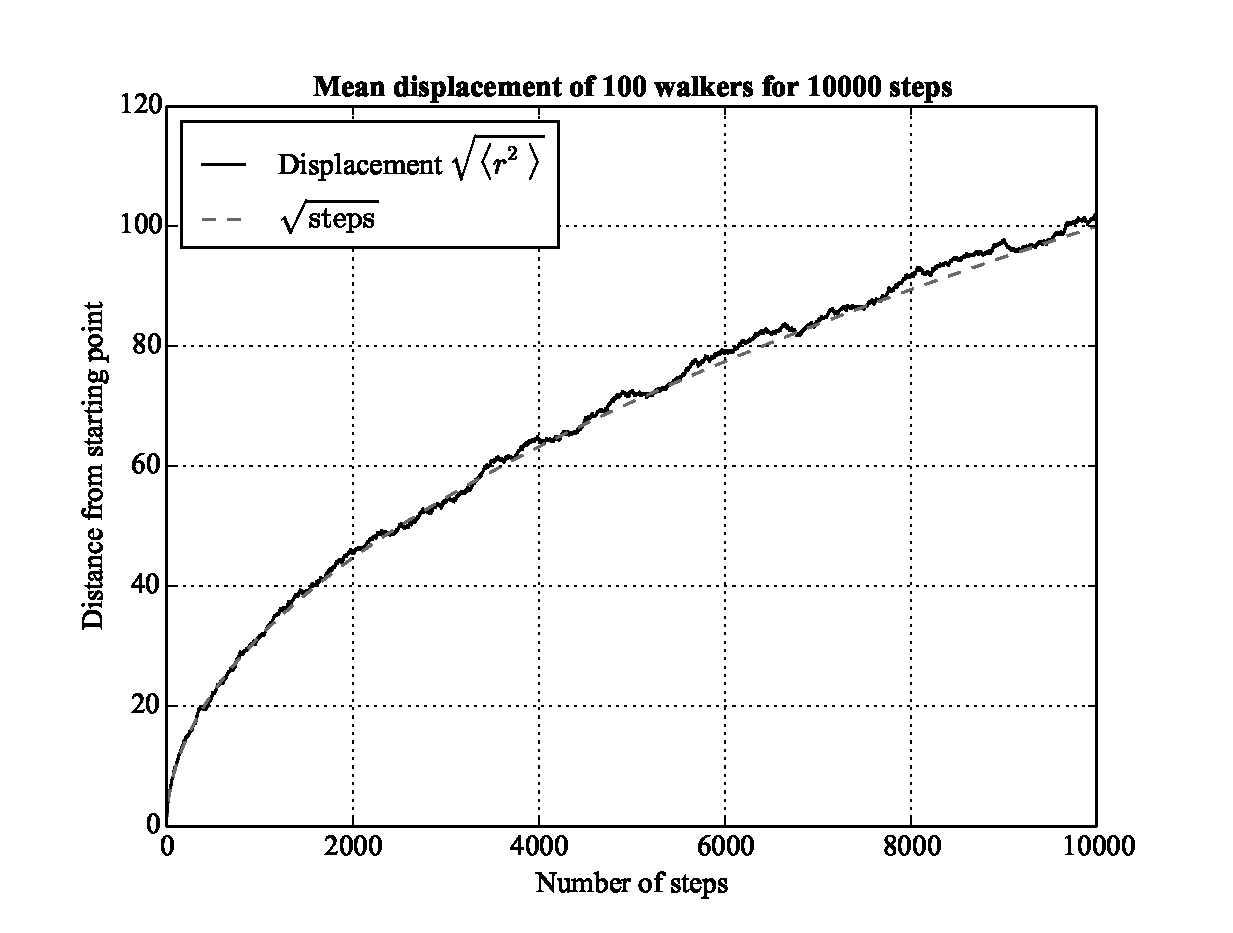
\includegraphics[width=0.75\textwidth]{figures/md-figures/random-walk-mean-distance.eps}    
    \caption{Mean distance from starting point for all $N$ particles
        after $n$ steps.}
\end{figure}\label{fig:randomwalk}

\subsubsection{Limitations and Challenges}
The particles in our simulation are bound by the minimum image convention,
where each particle in the box has a `mirror particle' outside to
enforce periodic boundary conditions. Thus we can't measure the
real displacement unless we take this into account.
One way to solve the problem is to give the particles
a displacement property $d$, a three-dimensional vector, 
whcih keeps track of the displacement.
The displacement is then updated in the same way as the
position in the velocity verlet algorithm
\begin{equation}
    d_{i+1} = d_i + v_{i+1/2}\Delta t
\end{equation}
With this solution, we are also free to set the initial position $d_0 = 0$,
instead of keeping track of $r(0)$ for every particle.
The periodic boundary conditions are not enforced on the displacement
vector, and has no impact on the system---it just records the mean 
displacement while $r_i$ is the particle position.

We still have to correctly initialize the system and thermal equilibrium is
needed before we start recording the mean displacement.
It is also important to initialize the system in the correct phase.
If we look at a system of a solid, there won't be much to diffusion to be seen.

In a nano-porous system it is not obvious how we could measure the
mean displacement. In the nano-porous system we have some closed-off
pores and the particles in these won't contribute to the transport through
the system. Should we then focus only on the particles that are
able to go from one side of the system to the other?


\invisiblesubsection{Measuring the Radial Distribution}
\setcounter{subsubsection}{0}
\newpage
\begin{tcolorbox}[title = Measuring the radial distribution] 
    How can you measure the radial distribution function?
    What does it tell? What challenges will you face?
    compare the measurement of the radial distribution function
    to the measurement of the probability densities for a
    random walk.
\end{tcolorbox} 

\subsubsection{The Radial Distribution Function}
Consider a particle in our system. 
The \ita{radial-distribution function}---also known as 
the \ita{pair-correlation function}---$g(r)$ 
is the probability that we will find another particle some distance $r$
away from our reference.
If we imagine a shell around the particle, the distribution function is
the density of that shell with radius $r$.
One could measure this distribution by counting all particles
in the shell for increasing $r$.
The distribution is normalized with respect to uncorrelated particles,
in other words an ideal gas,
\begin{equation}
    \lim_{r\rightarrow\infty} g(r) = 1
\end{equation}
The local time-averaged particle density is then found as $\rho g(r)$.

\subsubsection{Measuring the Distribution Function}
The fundamental properties that we have in our simulations
are the positions and velocities of every particle.
To measure the radial-distribution function $g(r)$, we
have the following procedure\footnote{See below the procedure
for a more effective method.
},
\begin{itemize}
    \item Choose a reference particle
    \item Calculate the distances to all other particles
    \item Bin the distances appropriately
    \item Create a histogram that is an estimate for $g(r$)
\end{itemize}
If we do this procedure with all particles as references,
and take the average,
we will have a good estimate. To this more efficiently,
we should instead calculate the distances between all particle-pairs,
bin them, and then create the histogram.
We must remember to divide by the volume, since we are interested in the
particle density we are interested in.

\subsubsection{Using the radial-distribution function}
We can measure the distribution function experimentally
by looking neutron and x-ray scattering of matter,
and thus verify the numerical methods.

The structure of the system we are looking at tells us what kind
matter we are looking at. Fluids will have other forms
than solids. Therefore the distribution function
gives us information about the average particle density
and therefore the type of structure.
A solid will for example have a typical lattice formation,
and the system of Argon atoms that we looked would
give us clear spikes---defining the FCC lattice structure we used---with
just small vibrations.
Increasing the temperatures gives the particles
larger kinetic energies, and the spikes will be broader.
Even higher temperatures, such that the system becomes a gas,
will yield a spike at the beginning and less form as the radius increases.
The reason for the first spike is the strong repulsive 
forces for small distances.

The radial-distribution function lets us see a link between the
macroscopic and microscopic properties of the matter.
This is due to our use of microscopic information to say something about
the macroscopic properties.

\subsubsection{Challenges}
Computing the distribution function is computationally intensive.
We loop over all particle pairs, and thus incur $\mc O(N^2)$ operations
and a large dataset. Doing this for many time-steps is costly operation-wise.
To counter this, we could use the approach of cut-off distances:
for some $r > r_{\text{cut}}$ we stop doing the calculations.
In this case, we assume that distances past $r_{cut}$ implies
$g(r)\sim 1$.
The already integrated cell-list functionality for force-calculations
can then be used to achieve this.

If we choose bin sizes that are too small, we might divide by a very small
volume and obtain errors because of machine representation of floating point
numbers. It might be difficult to know how to choose the bin sizes.
One could do it linearly with respect to $r$, or some exponential of $r$.

\invisiblesubsection{Thermostats}
\setcounter{subsubsection}{0}
\newpage
\begin{tcolorbox}[title = Thermostats] 
    Discuss the microcanonical versus the canonical ensemble
    in the simulations. How can we obtain results from a
    canonical ensemble? Introduce two thermostats, and
    describe their behavior qualitatively. How can you use
    such a thermostat for rapid initialization of a
    microcanonical simulation?
\end{tcolorbox} 

\subsubsection{The Canonical Ensemble and Thermostats}
The microcanonical ensemble describes a system where the
volume $V$, number of particles $N$ and total energy $E$ is held constant.
This is different to the canonical ensemble where the system is permitted
to exchange energy, but the temperature $T$ is held constant.
Generally in molecular dynamics, we want to study a microcanonical ensemble.
However, sometimes it is of interest to simulate the canonical ensemble.
To achieve this we need something to keep the temperature constant.
We use a thermostat to do this: an external heat 
bath in contact with our system.

A thermostat should satisfy some requirements:
\begin{enumerate}
    \item It should be able to control the temperature of the system
        such that it is close to the temperature of the heat bath.
    \item It should not disturb the system dynamics, and it should
        sample the quantities of the phase space (positions and velocities).
    \item It should be adjustable.
\end{enumerate}

Our best bet for a thermostat that satisfies these demands is the
\ita{Nosé-Hoover thermostat}.
We have already discussed this thermostat, so we'll look at
two others instead.

\subsubsection{The Berendsen Thermostat}
Many thermostats rescale the velocities of the systems' particles
by a factor $\gamma$. One of these is the \ita{Berendsen thermostat}.
The scaling factor is
\begin{equation}
    \gamma = \sqrt{1+\frac{\Delta t}{\tau}\left(
            \frac{T_{\text{bath}}}{T} - 1    
        \right)}
\end{equation}
Here $\tau$ is called the \ita{relaxation time}: which lets us
adjust the (weak) coupling to the heat bath. A greater $\tau$ value gives
a weaker coupling.
This means that the Berendsen thermostat works by dampening the
fluctuations of the systems' kinetic energy.
The velocity scaling is such that change in temperature is proportional
to difference in temperature between the heat bath and the system.
\begin{equation}
    \Delta T = \frac{\Delta t}{\tau}(T_0 - T(t))
\end{equation}

The thermostat is not able to represent a correct canonical ensemble,
but for large enough systems, we will achieve approximately
correct results.
It is often used because it effectively thermalizes the system to
the temperature of the heat bath,
and can be used to initalize a system before applying the Nosé-Hoover
thermostat.

\subsubsection{The Andersen Thermostat}
Another simple thermostat is the \ita{Andersen thermostat}.
It works by simulating collisions between particles in the system
and in the heat bath.
For every particle in the system we generate a random number
uniformly generated between 0 and 1.
If the number is less than $\sfrac{\Delta t}{\tau}$,
we let the particle be one of the colliding particle. 
Thus the particle needs a new velocity, which is
generated from a Boltzmann distribution with standard deviation
$\sqrt{k_B T_{\text{bath}}/m}$.
We can adjust the thermostat by changing $\tau$, which can
be considered the \ita{collision time}.
The collision time describes the strength of the coupling beween
the system and the heat bath.

Assuming ergodicity, the Andersen thermostat gives us
a canonical distribution of microstates.
The Algorithm is non-deterministic and thus not time-reversible.
It should only be used when measuring time-independent properties.
Diffusion, which is something we have looked at, should not be
calculated if the system has been influenced by the Andersen thermostat.

The thermostat is useful for equilibrating the system,
but disturbs the natural vibrations of the crystal structure.

In project 1 we experienced that the Berendsen thermostat gave smaller
fluctuations in the system than the Andersen thermostat.

\newpage
\section{Advanced Molecular Dynamics} 
\setcounter{subsection}{6}
\invisiblesubsection{Generating a Nanoporous Naterial}
\setcounter{subsubsection}{0}
\begin{tcolorbox}[title = Generating a Nanoporous Material]
    Discuss how we prepare a nanoporous matric with a given
    porosity. How do we characterize the structure of such 
    a material and the dynamics of a fluid in such a material?
\end{tcolorbox}

\subsubsection{Simulating Nanoporous Materials with MD}
Nanoporous materials are porous materials with pores
less than $\sim 100 $ nanometers.
We want to simulate fluids going through the pores of the material
and so we need to create a solid matrix with pores.
The solid material is then filled with a fluid, and
we can do normal MD measurements on it.
It could for example be a Silicon dioxide block with water in it.

\subsubsection{Generating the Solid Matrix}
We usually generate the matrix in the `opposite' way of what an
experimental physicist would do.
By creating a bulk material of for example Argon, and then
`freezing' part of it so it becomes a solid, while the
rest of the atoms are kept liquid.
In percolation theory we have a probability $p$ of which atoms
to freeze. This would give us too small pores, so we should use another
approach. Like a pumpkin, we could carve out parts of the
solid---either with randomly distributed spherical pores of some radius
or using cylindrical pores---removing the atoms 
(either the ones inside or outside the spheres) until we have
the wanted porosity. An approximation to the porosity is
the ratio between the particles inside and outside the spheres,
$\phi = 1 - N_{\text{matrix}}/N (= V_{\text{pore}}/V)$,
since the porosity is the relative part of the total pore-volume.
The fluid is then the atoms which have not been frozen,
and we should reduce the density of these.

\subsubsection{Characterizing the Material-structure 
    and Dynamics of the Fluid}
The fluid in the system can be characterized by
two properties:
\begin{itemize}
    \item Porosity $\phi$: The ratio between pore-volume and
        total volume.
    \item Permeability $k$: The ability of a fluid to travel
        through the porous medium. It is a function of
        the size of the pores, the connection between pores
        and the tortuosity of the medium.
\end{itemize}

The permeability $k$ is measured by simulating the flow through the
system. We do this by applying a pressure difference to the system.
The permeability is affected by the porosity which allows transfer,
the size of the pores, and the amount of twists and turns:
the \ita{tortuosity}.

In addition to the above properties, which are properties of
the material, the flow also depends on the properties of the
fluid, for example the density.

We can measure the flow by asserting a pressure gradient $\nabla P$,
and the flow is described by \ita{Darcy's law}\footnote{The 
    derivation of this expression comes from the simplified
    Navier-Stokes equation (`Stokes equation'),
    \url{https://en.wikipedia.org/wiki/Darcys\_law\#Derivation}},
\begin{equation}
    U = \frac{k}{\mu}(\rho g - \nabla P)
\end{equation}

where $\rho g$ is the gravitational part. The pressure gradient
is from hydrostatic conditions. $\mu$ is here the viscosity
of the fluid. 

To generalize this to our needs, we
rewrite the gravitational term to a global force by
\begin{equation}
    \rho g = \frac{N}{V} mg = \frac{N}{V} F_g = n F_g
\end{equation}
We can now switch out the gravitational force $F_g$ by
a general force-term $F_x$. We dub the number of particles
per volume as the \ita{number density} $\sfrac{N}{V} = n$.
If we ignore the pressure gradient, our equation now reads
\begin{equation}
    U = \frac{k}{\mu}n F_x
\end{equation}

To find the remaining unknowns, we look at the known velocity profile
for a cylindrical pore of length $L$ and radius $a$,
\begin{equation}
    u(r) = \frac{\Delta P}{L} \frac{1}{4\mu}(a^2 - r^2)
\end{equation}
By creating a system with only one of these pores, we can 
calculate the viscosity $\mu$. We'll have to let the system reach
equlibrium before we do the measurements, of course.
This is when the particles on average is no longer accelerated,
and the temperature only has small fluctuations. This
could take some time. The velocity profile is then
measured by splitting the radii into bins, finding the mean
velocity and then dividing by the number of particles in the respective bin.
This is plotted in a histogram.

If we now keep the same density $\rho$ in our actual system,
we should be able to use this $\mu$ in our calculations
(since the viscosity is fluid dependent).
Then we can find the permeability as
\begin{equation}
    k = \frac{U\mu}{n F_x}
\end{equation}


\invisiblesubsection{Diffusion in a nanoporous material}
\setcounter{subsubsection}{0}
\newpage
\begin{tcolorbox}[title = Diffusion in a nanoporous material]
    How can you measure the diffusion constant for a low-density
    fluid in a nanoporous system? Discuss what results you expect.
    Compare with diffusion in a bulk liquid and in a
    larger-scale porous medium.
\end{tcolorbox}

\subsubsection{How to Measure the Diffusion Constant}
Diffusion is the process of particles mixing due to their random motion.
It's described by Fick' law
\begin{equation}
    J = -D \frac{\partial\phi}{\partial x}
\end{equation}
with $D$ as the diffusion constant/coefficient.
In physics terms it's the proportionality factor between
the concentration gradient and the net diffusion flux.

In our MD system there isn't a concentration gradient
and thus no net flux. However, there is an internal microscopic
motion of the particles, a self-diffusion in the system.
If we look at a single particle, it will not tend to move in a
general direction, so the expected value of the position is zero,
$\langle r \rangle = 0$. Though the particle doesn't have a
tendency to move in some direction, the actual distance travelled
is not zero. Therefore the \ita{mean displacement} 
is a measure of this quantity, given by $\langle r^2 \rangle (t)$.

The macroscopic diffusion can be predicted since it is the motion
of all the individual particles in a gas. To model this,
we use \ita{random walkers}. A walker is a model of a single
particle, discretized to take steps in some directions.
For each step, it has a probability to move in some direction or another.
The displacement of a single walker 
is then the sum of the displacements $\vec x_i$ of all the $n$ steps,
\begin{equation}
    \vec X_n = \sum_{i=1}^n \vec x_i
\end{equation}
We can study this system both analytically and through Monte-Carlo
simulations. For most probability distributions of $x_i$,
we let it be symetrical, such that the probability for a step
in any direction is equal. When the distribution
is symmetric, it is easy to show that the expected displacement
is zero and that the mean displacement is proportional to the number of steps,
\begin{equation}
    \langle \vec X_n \rangle = 0,\;\;\; \langle \vec X_n^2 \rangle \propto n
\end{equation}

A walker that moves in $d$ dimensions, for example a particle in a box,
has a proportionality factor of $2 d\cdot D$.
In a Monte-Carlo simulation with a large number of
random walkers moving in a box with a concentration gradient,
we predict the diffusion from the random distribution.

The random walk model is of course different from our system,
in that the particles do interact. Luckily this doesn't matter,
and the interesting part is the mean displacement.
The fact that particles interact is embedded into 
the measure of the displacement.
Because the system consists of a large number of particles,
we expect that the particles average (squared) displacement
estimates the expectancy of a single particle (squared) displacement
in a good way.

In a nanoporous system, we actually have the \ita{same}
result. The interactions affect the mean-square displacement,
but it is only a mathematical fact of the connection
between the microscopic mean displacement and the macroscopic diffusion.
In our calculations we leave out both the solid matrix and
the particles trapped in pores which aren't connected---and thus
can't diffuse anywhere. Since the particles are allowed to move
in a smaller area, the mean displacement is also smaller.
This means that the diffusion constant must also be smaller,
which is reasonable since it's harder to move through tunnels
than open space. One can think of it as the dimension value $d$
is less than 3, though we have three dimensions (thus the
$D$ value is still the same). This behavior is amplified
with smaller pores.
The diffusion might also vary in the dimensions.
Though, if we randomly distribute the pores, these differences should
disappear when the system size increases.

We trace the motion of every atom and can therefore estimate the
diffusion constant from the mean displacement squared 
(in one dimension)\footnote{The mean displacement squared in three
    dimensions is of course
    $\langle r^2 \rangle 
    = \langle x^2 \rangle + \langle y^2 \rangle + \langle z^2 \rangle$.
}
from all the particles by
\begin{equation}
    \langle x^2(t)\rangle 
    = \frac{1}{N}\sum_{i=1}^N {(x_i(t)-x_i(0))}^2
\end{equation}

By plotting the mean distance, we can find the slope by linear regression
to estimate the diffusion constant $D$ since they are proportional. 
Figure~\ref{fig:randomwalk} shows us that the mean distance from the starting
position of all walkers is proportional to 
$\sqrt n$. We will not see this behavior
for only one walker---thus increasing the number of walkers
will make the curve approximate $\sqrt n$.

\subsubsection{Expectations}
Studying precolation systems has given us a greater intuition
for diffusion in nanoporous materials.
We see that the systems can either have diffusion through
the whole system or only in some parts, if the
pores are closed off from each other.
Diffusion through the whole system is also governed by the size 
and form of the pores.

The diffusion coefficient in a nanoporous system should always
be smaller than in a bulk solid. Random motions in an
`open' area will disperse more since it's easier than
maneuvering through tunnels.
We must thus have an \ita{effective} diffusion constant
that takes into account the factors in a nanoporous material.

The first to take into account is the \ita{transport-available}
porosity $\epsilon_t$: the porosity that actually leads from one side to
the other---or in others words the porosity avilable for macroscopic transport
of fluids.
It is the total volume withough the solid matrix, the pores that are too
small, dead ends and the pores that are sealed off from the rest of the system.

The second is the \ita{constrictivity} $\delta$.
As our system consists of nanoscopic pores, there is a large contribution
from surface tension along the walls. This results in a higher viscosity
as the fluid has more trouble moving close to walls.
The constrictivity is dependent on the size of the particles in the fluid
and the pore size.
It is a dimensionless scaling paramter and since the diffusion is less
than in a bulk material, we have $\delta \leq 1$.

The final thing to consider for the effective diffusion coefficient is
the curve-number of the pore tunnels. 
This is called the \ita{tortuosity} $\tau$, and is the number of turns
a curve has, thus for a porous system we have $\tau > 1$.
A system with many twists and turns will therefore have lower diffusion.

The effective diffusion coefficent can now be written
\begin{equation}
    D_e = \frac{D\epsilon_t \delta}{\tau}
\end{equation}
and we see that each of the terms lowers the diffusion independently of
the others.

\subsubsection{Comparison Between Bulk Liquid and Large-scale Porous Medium}
The three systems of bulk liquid, larger-scale porous systems
and nanoporous systems will all have diffusion. However the rate of
diffusion will vary between the three. They all have a 
mean square displacement that will be proportional to time.
The diffusion coefficient will be different, but they all
respect Fick's law of mass transportation.

As explained earlier, we expect the diffusion coefficient of
a bulk liquid to be greater than that of porous media, as
we have $e_t < 1$, $\delta \leq 1$ and $\tau \geq 1$.
Since downscaling a porous system to a nano-scale system
will give less space in every pore, the constricitivity will be
smaller, $\delta_{np} < \delta_p$. It is also possible
that the tortuosity will be larger, as smaller pores could mean
more tunnels and so we might have more turns, $\tau_{np} > \tau_p$.


\invisiblesubsection{Flow in a nanoporous material}
\setcounter{subsubsection}{0}
\newpage
\begin{tcolorbox}[title = Flow in a nanoporous material]
    Discuss how to induce flow in a nanoporous material.
    How can you check your model, calculate the fluid viscosity
    and measure the permeability? What challenges do you expect?
\end{tcolorbox}

\subsubsection{Generating the Nanoporous Matrix}
To induce flow in a nanoporous material, we must first
create the matrix. We did this by creating a bulk Lennard-Jones fluid system,
`froze' all the particles and carved out pores of spheres
obeying a random distribution, until we were satisfied with
the porosity: the ratio between pore volume and the total system volume.
We could now fill the matrix with a fluid, either of the same
atoms as the solid, or any others.
In our project we used the same Lennard-Jones fluid as the solid,
but at half the density. Though the solid is frozen, the atoms
contribute to the force calculations, but since they don't move,
they are ignord in the integration of the equations of motion.

\subsubsection{Flow: inducement and measurements}
The pores can either be connected or separated, but if they
are connected, the fluid can move from one side to the other---a
macroscopic flow through the system.
In the microcanonical ensemble, we didn't have a flow, as 
there was no pressure gradient in the system.
By adding a global force to the system, we can create a pressure
gradient and measure the induced flow.

By Darcy's law, we have
\begin{equation}
    U = \frac{k}{\mu}(\rho g - \nabla P)
\end{equation}
$U$ is the volume flux per area per time. $k$ is the permeability,
the ability for the fluid to flow through the system.
$\mu$ is the viscosity, the `thickness' of the fluid,
or how well it resists changes.
$\rho g$ is the gravitational term, which is the force
that cause movement in the fluid. Finally we have the
pressure gradient $\nabla P$ which usually comes from hydrostatic
conditions\footnote{\ita{Hydrostatics} is the study of incompresible
    fluids at rest (opposed to \ita{fluid dynamics}).}.

We are not interested in the gravitational forces,
so we replace it with a global force by
\begin{equation}
    \rho g = \frac{N}{V} mg = \frac{N}{V} F_g = n F_g
\end{equation}
In our system, we don't have hard walls, only periodic
boundary conditions, so we can remove the hydrostatic build-up of pressure,
\begin{equation}
    U = \frac{k}{\mu}n F_x
\end{equation}
We can then let the force $F_x$ affect the system over time and measure
$U$. The measurement must be done when the flow is stationary, 
which means that the particles on average is not under acceleration,
and the temperature only has small fluctuations.
The remaining unknowns are permeability $k$ and viscosity $\mu$.
We must find the ratio between these, as we can't measure them independently.

\subsubsection{Viscosity and Permeability Measurements}
There are systems where we know the permeability. One
of these is where we only have \ita{one} cylindrical pore,
with radius $a$, length $L$ and pressure difference between each side
$\Delta P$.
We expect this system to have the velocity profile
\begin{equation}
    u(r) = \frac{\Delta P}{L} \frac{1}{4\mu}(a^2 - r^2)
\end{equation}
at stationary flow. The pressure difference is 
$\Delta P = n F L$, so $\Delta P/L = nF$.
This shows that the flow is fastest in the middle of the cylinder.
Near the walls we have virtually no flow, due to the interactions
between walls and fluid.

We measure the velocity profile at stationary flow by splitting 
the radii into bins, finding the mean
velocity and then dividing by the number of particles in the respective bin.
This is plotted in a histogram, and we can measure the
viscosity $\mu$.

If we now keep the same density $\rho$ in our actual system,
we should be able to use this $\mu$ in our calculations
(since the viscosity is fluid dependent).
Then we can find the permeability as
\begin{equation}
    k = \frac{U\mu}{n F_x}
\end{equation}

\subsubsection{Challenges}
The viscosity $\mu$ is as stated fluid dependent, and changing the
density will therefore alter the viscosity.
It can take a while to reach stationary flow (steady state),
and this \ita{must} be done in order to get correct results.
The flux value $U$ must be measured consistently.
We can't in one moment measure the volume flux, and in the next
measure the area and time flux.

\newpage
\section{Percolation}
\setcounter{subsection}{9}
\invisiblesubsection{Algorithms for percolation systems}
\setcounter{subsubsection}{0}
\begin{tcolorbox}[title = Algorithms for percolation systems]
   How do we generate a percolation system for simulations?
   How to analyze and visualize the systems? 
   How to find spanning clusters and measure the percolation probability?
\end{tcolorbox}

\subsubsection{Generating the Percolation System}
We generate a percolation system numerically by creating a matrix lattice
of size $L\times L$ (or a 1D system of length $L$) 
with elements randomly chosen between 0 and 1.
We then check each \ita{site} on the lattice and create a new
matrix. If the points are larger than some probability $p$, 
the point is occupied
and we set the value to 1. Otherwise we set the value to zero.
The probability for a site to be unoccupied is $q=1-p$,
and the process is uncorrelated between sites.
For two sites to be connected, we use the `nearest
neighbor' rule which means that in two dimensions we
have four candidates per site (except on the boundaries).

\subsubsection{Analysis and Visualization}
The system can be visualized by plotting a grid with
colored (black and white) squares for each occupied or
unoccupied state. For percolation to occur, we must
have a path that leads from one side to the other.
That is, there must be neighboring squares all the way across.

A set of neighboring squares is called a \textit{cluster},
and a cluster that spans all the way across is a \textit{spanning} 
cluster. The percolation \ita{threshold} $p_c$ is when
we get a spanning cluster, or in other words: a percolationg system.
For an infinite system, this value is set, but
for finite systems, we have a new $p_c$ for each realization.

To find a spanning cluster in a percolation system,
we must first find the clusters in the system.
This is done by checking all neighbors of a square
and labeling them with a number.
This can be done with automated methods in Python or MATLAB,
but we can also write a brute-force algorithm.

When all sites are given a label, we can plot the matrix
with each cluster having a distinct color. The colors should
be randomized so it's easier to separate the clusters (color
gradients are generally a bad idea).
For larger systems we will get a lot of clusters and so
it's even more important.

To check if a cluster is a spanning cluster,
we could implement a \ita{minimum bounding box}
around the cluster. That is a rectangle (in two dimensions)
that encloses all the sites. If either the width or height
of the rectangle matches the length $L$, we have a spanning cluster.
Fig~\ref{fig:min-bound-box} shows this.

\begin{figure}[h]
    \centering
    \includegraphics[width=0.40\textwidth]{figures/percolation-figures/minimum-bounding-rectangle.pdf}    
    \caption{An example of a minimum bounding box.}\label{fig:min-bound-box}
\end{figure}

The minimum bounding box is well-suited for $L\times L$ geometries,
but not so much for more complicated ones.
For these geometries it is better to look at the set of clusters
that borders one side, and another set that borders the other.
The intersection between these two sets is the set that contains
our spanning clusters.

\subsubsection{Percolation Probability}

The probability of there being a spanning cluster in the
system is given by the percolation probability $\Pi (p, L)$.
If we generate one matrix, and checks if it percolates, 
we of course have the answer: yes or no.
Therefore we must do many experiments to find out
the percolation probability.
We can find this probability in a set of finite systems
by counting the number of times a set of random lattices
percolate for different p values. That is:

\begin{enumerate}
    \item Choose the number of experiments $N$.
    \item Create a set of random lattices 
        and check if they percolate for
        a set of values $p_i$.
    \item $N_i$ is the number of percolating systems we have for
        a given $p_i$.
    \item Then we have $\Pi(p_i, L) = \sfrac{N_i}{N}$.
\end{enumerate}

As the length $L\rightarrow \infty$, the percolation probability
should become 1 after some $p = p_c$, the \ita{percolation threshold}.
For a 1D system, this is of course when $p=1$, since we only have
percolation when all sites are filled.

\invisiblesubsection{Percolation on small lattices}
\setcounter{subsubsection}{0}
\newpage
\begin{tcolorbox}[title = Percolation on small lattices]
    Discuss the percolation problem on a $2\times2$ lattice.
    Sketch $P(p,L)$ and $\Pi(p,L)$ for small L.
    Relate to your simulations. How do you calculate
    these quantities and how do you measure them in simulations?
\end{tcolorbox}

\subsubsection{Small Lattices}
We are interested in finding the percolation probability
$\Pi(p,L)$ and the cluster spanning density $P(p,L)$ 
for matrices of size $L\times L$.
The smallest $L$-values give us matrices that we can easily
draw and see what the probability and spanning cluster density is.
The results are analytic solutions (closed-form), but for
larger systems, it becomes difficult due to system size of 
$2^{L\times L}$.
We want to study these small systems anyway as they give clues
as to how the system sizes evolve, and thus we can 
relate them to results from numerical solutions for larger systems.

\subsubsection{Configuration of $2\times 2$ Matrix}

A $2\times2$ lattice can have 1, 2, 3 or 4 occupied states.
We can put the configurations into six groups like this:
\begin{figure}[h]
    \centering
    \includegraphics[width=0.50\textwidth]{figures/percolation-figures/2times2lattice-config.png}    
\end{figure}

If $p$ is the probability of an occupied state, then
for example $c=0$ has the probability $P(c) = {(1 - p)}^4$.
This is because we multiply the probability of there not
being a occupied state together four times.
The probabilities for all groups are given as:
\begin{table}[H]
    \centering
    \begin{tabu}{c c c c}
        \rowfont{\color{white}}
        \rowcolor{white!40!black}
        $\vec c$ & $\vec{g_c}$ & $\vec{P(c)}$ & $\vec{\Pi(p, L|c)}$\\
        \rowcolor{black!5!white}
        1 & 1 & $p^0{(1-p)}^4$ & 0\\
        \rowcolor{black!5!white}
        2 & 4 & $p^1{(1-p)}^3$ & 0\\
        \rowcolor{black!5!white}
        3 & 4 & $p^2{(1-p)}^2$ & 1\\
        \rowcolor{black!5!white}
        4 & 2 & $p^2{(1-p)}^2$ & 0\\
        \rowcolor{black!5!white}
        5 & 4 & $p^3{(1-p)}^1$ & 1\\
        \rowcolor{black!5!white}
        6 & 1 & $p^4{(1-p)}^0$ & 1\\
	\end{tabu}
			\caption{}\label{tab:perc-prob}
\end{table}

and the general expression is $p^x q^{4-x}$ where $x$ is the
number of occupied sites in the system.

The probability for a spanning cluster is\footnote{From probability
    theory we have $P(A) = \sum_B P(A|B)P(B)$, which implies 
    equation~\ref{eq:Pi-prob}.}
\begin{equation}
    \Pi(p,L) = \sum_c \Pi(p,L|c)P(c) 
    \label{eq:Pi-prob}
\end{equation}
and the probability $P(c)$ of spanning, given a configuration $c$,
is either 0 or 1, as we saw in table~\ref{tab:perc-prob}.
This leads us to the general equations
\begin{align}
    \Pi(p,L) &= 4p^2q^2 + 4p^3q + p^4\\
    P(p,L) &= 
    \frac{2}{4}\cdot 4p^2q^2 + \frac{3}{4}\cdot 4p^3q + \frac{4}{4}\cdot p^4
\end{align}
For the spanning cluster density, we must multiply each term of the
percolation probability by the size of the cluster for the given
configuration. The spanning cluster density is generally
$P = \sfrac{M_i}{L^2}$ where $M_i$ is the `mass' of the cluster.

Figure~\ref{fig:perc-small-L} shows us how $\Pi$ and $P$ behaves
for $L=2$. For the next few $L$-values, the curves are the same
only (gradually) more distinctive, the $\Pi$ curve is more S-shaped and
the $P$ curve is more curved.

Both curves increase from $p=0$ to $p=1$ and are smooth.
$P$ is however always below $y=p$. This is due to the fact that
the spanning cluster density is the probability that a random site
is part of the spanning cluster. The random site is not
always occupied, so we must have $p \geq P$. As the $p\rightarrow 1$,
the difference between the two vanishes.
Of course, for $L=2$, if there is a spanning cluster, all
occupied sites are part of the cluster, but in larger
systems we can have non-spanning and spanning clusters at the same time.

\begin{figure}[H]
    \centering
    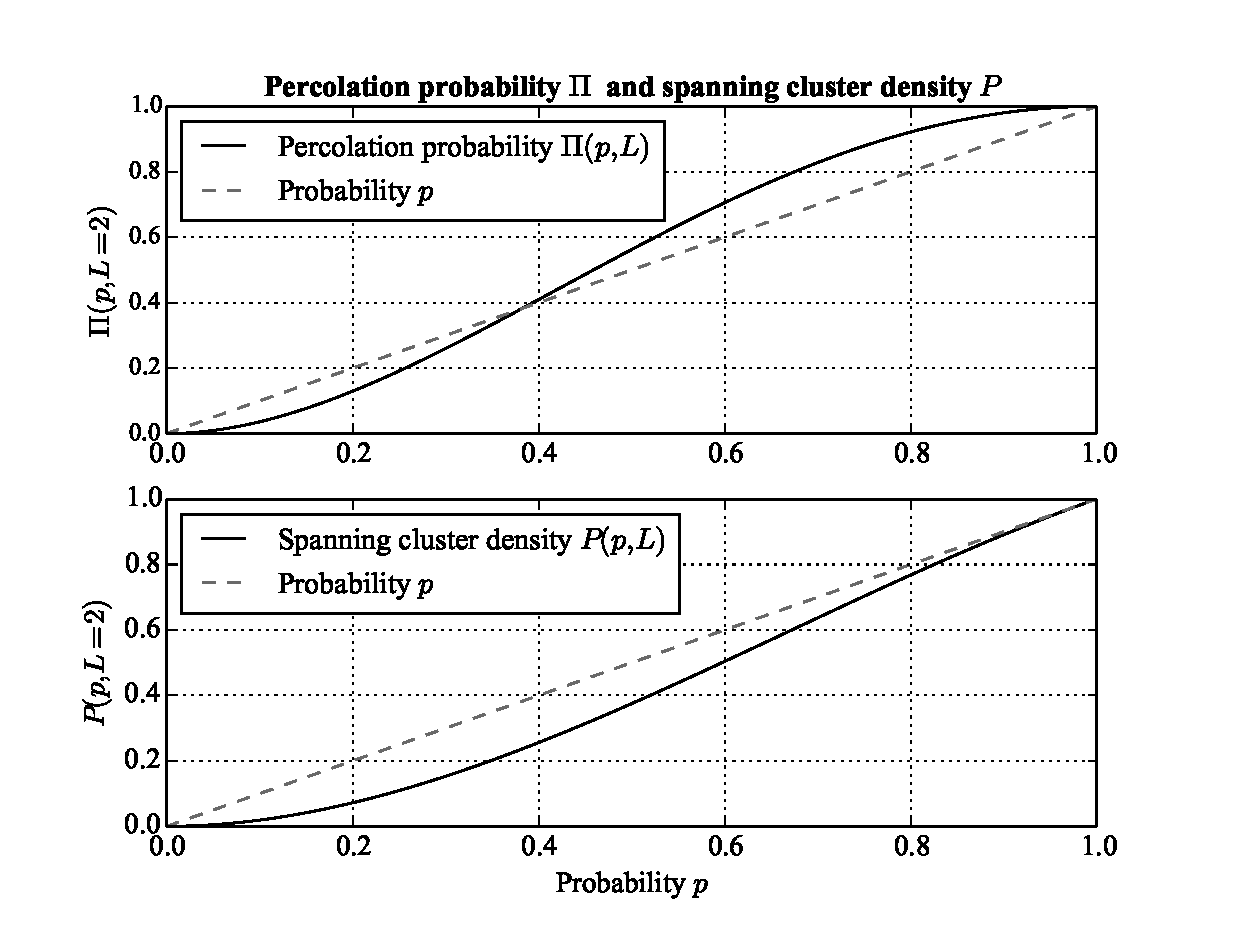
\includegraphics[width=0.75\textwidth]{figures/percolation-figures/perc-small-L.eps}
    \caption{Sketch of probabilities and cluster densities
        for $L=2$. The $y=p$ curve is the same as for
        $L=1$ in both cases. 
        For the next $L$-values (3 and 4) the curves are the
        same only more `dramatic'}\label{fig:perc-small-L}
\end{figure}

\subsubsection{Numerical Solutions of $\Pi$ and $P$}
The size of a two-dimensional percolation system is $2^{L\times L}$.
For larger systems, we can't manually find the
the analytical solutions of $\Pi$ and $P$.
However, we can find them using Monte-Carlo methods.
We generate $N$ matrices of size $L\times L$ and
check if they percolate or not. $n$ is the number of
matrices that do percolate. Each system has a mass of $M_i$,
and thus we estimate $\Pi$ and $P$ as
\begin{equation}
    \Pi(p,L) = \frac{n}{N},\;\;\; P(p,L) = \frac{\sum_i M_i}{NL^2}
\end{equation}

\invisiblesubsection{Cluster number density in 1D percolation}
\setcounter{subsubsection}{0}
\newpage
\begin{tcolorbox}[title = Cluster number density in 1D percolation]
    Define the cluster number density for 1D percolation,
    and show how it can be measured. Discuss the behavior when 
    $p\rightarrow p_c$. How does it relate to your simulations
    in two-dimensional systems?
\end{tcolorbox}

\subsubsection{Definition}
A 1D system will only percolate if all sites are occupied,
like water through a pipe will only if flow if there are no 
obstacles. 

Imagine a cluster of size $s$ in a 1D pipe.
A specific site in the cluster could be the first site from 
the left. The probability for a site to belong to a
specific site in a cluster of size $s$ is called the
\ita{cluster number density}, given by $n(s,p)$.

The probability of a site being occupied is $p$.
For all other sites in the cluster to be occupied, we have
the probability $p^{s-1}$. Now we also need to make sure that
these points are actually grouped together. The sites on each side of
the cluster has a probability of $1-p$ of being unoccupied.
Thus the cluster number density is
\begin{equation}
    n(s,p) = {(1-p)}^2 p^s
\end{equation}

These probabilities need to be summed the number of sites
in the cluster, namely $s$. 
Thus, if we point at a specific site in a cluster in a lattice, the
probability of that site to be part of a cluster of size $s$ is
\begin{equation}
    P(\text{site is part of cluster of size s}) = s\cdot n(s,p)
\end{equation}

\subsubsection{Measurements}
Given a finite system, we can count the number of
clusters of size $s$ as $N_s$. The size of the system is
$L$, so in a simulation we can measure the \ita{estimated} 
cluster number density $\bar n$ 
as\footnote{In $d$ dimensions, we have 
    $\overline{n(s,p)} = N_s/L^d$}
\begin{equation}
    \overline{n(s,p)} = \frac{N_s}{L}
\end{equation}

We can improve the estimate by generating $M$ different systems
and estimate the average
\begin{equation}
    \overline{n(s,p)} = \frac{N_s}{L M}
\end{equation}

Large systems yield very different $s$-values, but we
can bin them and create a histogram.
We should however create logarithmic bin sizes,
so the bin-width increases as $s$ increases.
Else we would get a lot of empty bins.
It is now very important to divide every bin with the correct
bin size.

\subsubsection{Convergence Behavior for $p\rightarrow p_c$}

A one-dimensional pipe has to have all sites occupied in order
to percolate. For an infinitely long pipe, 
the threeshold probability is thus $p_c = 1$.

To see the behavior when $p\rightarrow p_c$, we begin
by creating the function
\begin{equation}
    G(s) = \frac{n(s,p)}{{(1-p)}^2} = p^s
\end{equation}

If we plot this (see below), we see that as a function of $s$,
the cut-off is increased when $p\rightarrow 1$.

Let us now visualize $G(s)$ in another way. We can rewrite
\begin{equation}
    n(s,p) = {(1-p)}^2e^{s\ln p} 
    = {(1-p)}^2 e^{\sfrac{-s}{s_{\xi}}}
\end{equation}

where we have defined $s_{\xi} = \sfrac{-1}{\ln p}$.
The result is plotted below, and we now see that when we rescale
the $s$ axis, we align the graphs for different $p$ values.
We also notice that
\begin{equation}
    G(s) \rightarrow
    \begin{cases}
        1, &\text{if }s \ll s_{\xi}\\
        0, &\text{if }s \gg s_{\xi}\\
    \end{cases}
\end{equation}
This means that our system should have clusters of size
less than the characteristic cluster size,
but generally few that are larger.

As $p\rightarrow p_c = 1$, $s_{\xi} \rightarrow \infty$.
By using the Taylor expansion of $\sfrac{-1}{\ln p}$,
we can approximate it as
\begin{equation}
    s_{\xi} \simeq \frac{1}{1-p}
\end{equation}

This means that the divergence of $s_{\xi}$
is a power law with exponent $-1$ when $p\rightarrow 1$,
and it is the case for all dimensions.

We can now write the characteristic cluster size on general form
\begin{equation}
    s_{\xi} \propto {|p-p_c|}^{\sfrac{-1}{\sigma}}
\end{equation}
when $p\rightarrow p_c = 1$. 
In the one-dimensional case we have $\sigma = 1$.
The divergence is a property of the infinite system.

As $p$ approaches $p_c$, the infinite system is about to percolate,
so the cluster sizes increases. At one point, though,
we have a large (soon spanning) cluster that fuses with
the other large clusters and then the characteristic
cluster size drops in value again.

The $\sigma$ value is dependent on the lattice dimensionality,
and we can measure it by finding $s_{\xi}$ for $p$-values
close to $p_c$. We should see that it follows a power law.
This has the challenge that our system is finite,
so we could instead use the plot method from earlier.
When we plot as a function of $\sfrac{s}{s_{\xi}}$
we see that all the lines fall onto a single curve.
This is called a \ita{data-collapse}. 

In a two-dimensional case, we are able to distinguish between
the characteristic size $s_{\xi}$ (the mass) 
and the correlation length $\xi$.

\begin{figure}[H]
    \centering
    \includegraphics[width=0.75\textwidth]{figures/percolation-figures/cutoff-p-values.png}
\end{figure}

\invisiblesubsection{Correlation length in 1D percolation}
\setcounter{subsubsection}{0}
\newpage
\begin{tcolorbox}[title = Correlation length in 1D percolation]
    Define the correlation length $\xi$ for 1D percolation.
    Discuss its behaivor when $p\rightarrow p_c$.
    How is it related to cluster geometry and your results
    for two-dimensional percoaltion?
\end{tcolorbox}

\subsubsection{The Correlation Length}
The distance between two occupied sites $a$ and $b$ 
is denoted by $r$. These two sites are connected if all
sites in between (there $r$ are of them) are occupied.
The probability for this is called the correlation function
and in one dimension we have
\begin{equation}
        g(r) = p^r = e^{\sfrac{-r}{\xi}}
\end{equation}
where the \ita{correlation length} is $\xi = \sfrac{-1}{\ln p}$.
The correlation length can be seen as a cut-off variable
for the correlation function
\begin{equation}
    g(r)\rightarrow
    \begin{cases}
        1, &\text{if } r\ll \xi\\
        0, &\text{if } r\gg \xi
    \end{cases}
\end{equation}
In a given system we expect to find clusters of lengths up to $\xi$,
but seldom clusters larger than $\xi$.

\subsubsection{Divergence of the Correlation Length}
When the probability $p\rightarrow p_c = 1$, the number of sites
increases and thus $\xi$ diverges.

To study this better, we rewrite the correlation function as
\begin{equation}
    \xi = -\frac{1}{\ln p} = \frac{1}{1-p} =  {(p-p_c)}^{\nu}
\end{equation}

This is a general percolation result, 
where $\nu = 1$ in one dimension, and
$\xi\rightarrow \infty$ and diverges as a power law
when $p$ approaches $p_c$.
This is also the $p$-value where the spanning cluster forms.

\subsubsection{Cluster Geometry}
The correlation length $\xi$ is different from the
characteristic cluster size $s_{\xi}$, however this 
is only the case when we are beyond one dimension.
In one dimension length is the same as `mass'.
In two dimensions and above, a cluster of size/mass $s$
can have several different shapes, while in one dimension
it is always a straight line.
The correlation length gives us information about
the extent of the system, which is important
since the ratio $\sfrac{\xi}{L}$ determines
wheter the finite system affects the result.

When the correlation length is a lot smaller than the system
size, $\xi \ll L$, the effects of having a finite system
instead of an infinite is not noticeable.
The reason is that we don't have any clusters that are large enough
to ``notice'' that the system is finite.
However, when the system size is a lot smaller than the
correlation length, $\xi \gg L$ the systems behavior
is dominated by the the size of the system.
When $\xi\simeq L$, it is difficult to determine how close
we are to $p_c$, but we can estimate given
\begin{equation}
    L \simeq \xi \propto |p_c-p|^{-\nu}
    \Rightarrow |p_c-p| \propto L^{\sfrac{-1}{\nu}}
\end{equation}

The characteristic cluster size in dimensions $d$ is related
to the correlation length by
\begin{equation}
    s_{\xi} \propto \xi^D
\end{equation}
where $D$ is a fractal dimensionality constant $D<d$.

To quantify the geometry of clusters, we could look
at the maximum distance between any two points in the cluster,
or even the average distance between two points.
However, we wish to look at the
variance of the sites of the cluster to the centre of mass
of the cluster. It is similar to the standard deviation
We call this property the
\ita{radius of gyration}. For a given cluster $i$,
with size $s_i$, we can find the radius of gyration by
\begin{equation}
    R^2_i = \frac{1}{s_i}
    \sum_{j=1}^{s_i}{(\vec r_j - \vec R_i)}^2
\end{equation}

$R_i$ is the radius of gyration and $j$ is just a label for a given
site in the cluster. The cluster has a centre of mass $\vec R_i$
and for a site $j$, it's position in the cluster is $\vec r_j$.

The result is that a dense cluster of size $s$ will have
a smaller radius of gyration than a sparser cluster with
the same size, and
\begin{equation}
    s\propto R_s^D
\end{equation}



\invisiblesubsection{Cluster Size in 1D Percolation}
\setcounter{subsubsection}{0}
\newpage
\begin{tcolorbox}[title = Cluster Size in 1D Percolation]
    Introduce the characteristic cluster size for the 1D
    percolation problem, and discuss their behavior when 
    $p\rightarrow p_c$. Relate to your simulations on
    two-dimensional percolation.
\end{tcolorbox}

\subsubsection{Definition}
A 1D system will only percolate if all sites are occupied,
like water through a pipe will only if flow if there are no 
obstacles. 

Imagine a cluster of size $s$ in a 1D pipe.
A specific site in the cluster could be the first site from 
the left. The probability for a site to belong to a
specific site in a cluster of size $s$ is called the
\ita{cluster number density}, given by $n(s,p)$.

The probability of a site being occupied is $p$.
For all other sites in the cluster to be occupied, we have
the probability $p^{s-1}$. Now we also need to make sure that
these points are actually grouped together. The sites on each side of
the cluster has a probability of $1-p$ of being unoccupied.
Thus the cluster number density is
\begin{equation}
    n(s,p) = {(1-p)}^2 p^s
\end{equation}

These probabilities need to be summed the number of sites
in the cluster, namely $s$. 
Thus, if we point at a specific site in a cluster in a lattice, the
probability of that site to be part of a cluster of size $s$ is
\begin{equation}
    P(\text{site is part of cluster of size s}) = s\cdot n(s,p)
\end{equation}

With a little trick, we rewrite
\begin{equation}
    p^s = e^{s\ln p} = e^{\sfrac{-s}{s_{\xi}}}
\end{equation}
where $s_{\xi} = \sfrac{-1}{\ln p}$ 
is the characteristic cluster size.
It is the value of the largest cluster we can expect to find.
$n(s,p)$ is almost constant when $s < s_{\xi}$ but dies
out when $s > s_{\xi}$.
The probability $s\cdot n(s,p)$ still dies out, since
$s$ is linear and $n(s,p)$ vanishes exponentially when $s > s_\xi$.

\subsubsection{Convergence Behavior for $p\rightarrow p_c$}

The characteristic cluster size $s_\xi$ 
goes to infinity as $p$ approaches 1.
$p = p_c = 1$ is the percolation threshold for
1D percolation, and it is at this moment our system starts
percolating. When $p\rightarrow p_c$, the clusters
become bigger and bigger, but for an infinite system,
it won't percolate until $p=p_c$.

\subsubsection{Comparions with Two-dimensional Percolation}
The characteristic cluster size $s_\xi$ is the number of
sites in a cluster. In 1D this is the effectively length of
the cluster. When we proceed to two dimensions,
it is instead meaningful to separate the length from the size 
(or the mass if you want).
In one dimension the correlation length was found to
diverge as a power law.
We can now write the characteristic cluster size on general form
\begin{equation}
    s_{\xi} \propto {|p-p_c|}^{\sfrac{-1}{\sigma}}
\end{equation}
when $p\rightarrow p_c = 1$. 
In the one-dimensional case we have $\sigma = 1$,
and for larger dimensions, $\sigma < 1$.

This means that the characteristic cluster size diverges faster
in two dimensions than one.
As for the one-dimensional case, we won't see any
percolation until $p\geq p_c$. Before this, $s_\xi$ approached 
infinity, but after the threshold isreached, it goes back down.
This is due to the spanning cluster ``eating up'' the other
large finite clusters as $p$ increases past the threshold.
When $p\rightarrow 1$, the characteristic size approaches zero.
This is because $s_\xi$ describes finite clusters,
and the probability of finding a finite cluster is lower and
lower. Here the power law doesn't hold, as
it is only valid when $|p-p_c|$ is small.

\subsubsection{Cluster Geometry}
The correlation length $\xi$ is different from the
characteristic cluster size $s_{\xi}$, however this 
is only the case when we are beyond one dimension.
In one dimension length is the same as `mass'.
In two dimensions and above, a cluster of size/mass $s$
can have several different shapes, while in one dimension
it is always a straight line.
The correlation length gives us information about
the extent of the system, which is important
since the ratio $\sfrac{\xi}{L}$ determines
wheter the finite system affects the result.

When the correlation length is a lot smaller than the system
size, $\xi \ll L$, the effects of having a finite system
instead of an infinite is not noticeable.
The reason is that we don't have any clusters that are large enough
to ``notice'' that the system is finite.
However, when the system size is a lot smaller than the
correlation length, $\xi \gg L$ the systems behavior
is dominated by the the size of the system.
When $\xi\simeq L$, it is difficult to determine how close
we are to $p_c$, but we can estimate given
\begin{equation}
    L \simeq \xi \propto |p_c-p|^{-\nu}
    \Rightarrow |p_c-p| \propto L^{\sfrac{-1}{\nu}}
\end{equation}

The characteristic cluster size in dimensions $d$ is related
to the correlation length by
\begin{equation}
    s_{\xi} \propto \xi^D
\end{equation}
where $D$ is a fractal dimensionality constant $D<d$.

To quantify the geometry of clusters, we could look
at the maximum distance between any two points in the cluster,
or even the average distance between two points.
However, we wish to look at the
variance of the sites of the cluster to the centre of mass
of the cluster. It is similar to the standard deviation
We call this property the
\ita{radius of gyration}. For a given cluster $i$,
with size $s_i$, we can find the radius of gyration by
\begin{equation}
    R^2_i = \frac{1}{s_i}
    \sum_{j=1}^{s_i}{(\vec r_j - \vec R_i)}^2
\end{equation}

$R_i$ is the radius of gyration and $j$ is just a label for a given
site in the cluster. The cluster has a centre of mass $\vec R_i$
and for a site $j$, it's position in the cluster is $\vec r_j$.

The result is that a dense cluster of size $s$ will have
a smaller radius of gyration than a sparser cluster with
the same size, and
\begin{equation}
    s\propto R_s^D
\end{equation}

\subsubsection{Measurements}
Given a finite system, we can count the number of
clusters of size $s$ as $N_s$. The size of the system is
$L$, so in a simulation we can measure the \ita{estimated} 
cluster number density $\bar n$ 
as\footnote{In $d$ dimensions, we have 
    $\overline{n(s,p)} = N_s/L^d$}
\begin{equation}
    \overline{n(s,p)} = \frac{N_s}{L}
\end{equation}

We can improve the estimate by generating $M$ different systems
and estimate the average
\begin{equation}
    \overline{n(s,p)} = \frac{N_s}{L M}
\end{equation}

Large systems yield very different $s$-values, but we
can bin them and create a histogram.
We should however create logarithmic bin sizes,
so the bin-width increases as $s$ increases.
Else we would get a lot of empty bins.
It is now very important to divide every bin with the correct
bin size.

\invisiblesubsection{Measurements and Behavior of $P(p,L)$
    and $\Pi(p,L)$}
\setcounter{subsubsection}{0}
\newpage
\begin{tcolorbox}[title = Measurements and Behavior of {$P(p,L)$}
    and {$\Pi(p,L)$}]
    Discuss the behavior of $P(p,L)$ and $\Pi(p,L)$ in a system
    with a finite system size $L$. How do you measure these
    quantities?
\end{tcolorbox}

\subsubsection{Percolation Probability $\Pi$ and Cluster
    Spanning Density $P$}
$\Pi(p,L)$ is the percolation probability: the probability
that a randomly generated system of size $L$
has atleast one spanning cluster.
The spanning cluster density $P(p,L)$ is the probability
a given site has of being a part of the spanning cluster.
If we divide the average mass of a spanning cluster by
the number of sites in the system, we get the
spanning cluster density.
These properties are different for systems in one and two 
dimensions.

\subsubsection{Behavior of $\Pi$ and $P$}
For an infinite system, $L = \infty$,
there is a (dimension-specific) percolation threshold $p_c$
where the system \ita{always} starts to percolate.
For a one-dimensional system, which is basically a one
dimensional pipe, this threshold is of course when $p_c=1$.
In other words: all sites must be occupied, and they
are occupied with probability $p$.
In two dimensions this threshold is $p_c=0.59275$.
The percolation probability $\Pi(p,L)$ is then
a step function where $p_c$ is the point where
the probability of percolation goes from 0 to 1.
In the smallest system, $L=1$,
we have linear percolation probabilites---that
is $\Pi = p$ for both one and two dimensions.

For a small but finite $L$,
we are able to find analytical (closed-form) solutions
for the percolation probability.
In one dimension, it is as easy as
\begin{equation}
    \Pi(p,L) = p^L
\end{equation}
since every site is occupied with probability $p$
and all $L$ sites must be occupied.

In two dimensions, we can't find a general expression for
all $L$, but we can find it manually by listing
all the configurations as long as $L$ is small.
The system size grows exponentially as $2^{L\times L}$.

\subsubsection{Configuration of $2\times 2$ Matrix}

A $2\times2$ lattice can have 1, 2, 3 or 4 occupied states.
We can put the configurations into six groups like this:
\begin{figure}[h]
    \centering
    \includegraphics[width=0.50\textwidth]{figures/percolation-figures/2times2lattice-config.png}    
\end{figure}

If $p$ is the probability of an occupied state, then
for example $c=0$ has the probability $P(c) = {(1 - p)}^4$.
This is because we multiply the probability of there not
being a occupied state together four times.
The probabilities for all groups are given as:
\begin{table}[H]
    \centering
    \begin{tabu}{c c c c}
        \rowfont{\color{white}}
        \rowcolor{white!40!black}
        $ c$ & $g_c$ & $P(c)$ & $\Pi(p, L|c)$\\
        \rowcolor{black!5!white}
        1 & 1 & $p^0{(1-p)}^4$ & 0\\
        \rowcolor{black!5!white}
        2 & 4 & $p^1{(1-p)}^3$ & 0\\
        \rowcolor{black!5!white}
        3 & 4 & $p^2{(1-p)}^2$ & 1\\
        \rowcolor{black!5!white}
        4 & 2 & $p^2{(1-p)}^2$ & 0\\
        \rowcolor{black!5!white}
        5 & 4 & $p^3{(1-p)}^1$ & 1\\
        \rowcolor{black!5!white}
        6 & 1 & $p^4{(1-p)}^0$ & 1\\
	\end{tabu}
			\caption{}\label{tab:perc-prob}
\end{table}

and the general expression is $p^x q^{4-x}$ where $x$ is the
number of occupied sites in the system.

The probability for a spanning cluster is\footnote{From probability
    theory we have $P(A) = \sum_B P(A|B)P(B)$, which implies 
    equation~\ref{eq:Pi-prob}.}
\begin{equation}
    \Pi(p,L) = \sum_c \Pi(p,L|c)P(c) 
    \label{eq:Pi-prob}
\end{equation}
and the probability $P(c)$ of spanning, given a configuration $c$,
is either 0 or 1, as we saw in table~\ref{tab:perc-prob}.
This leads us to the general equations
\begin{align}
    \Pi(p,L) &= 4p^2q^2 + 4p^3q + p^4\\
    P(p,L) &= 
    \frac{2}{4}\cdot 4p^2q^2 + \frac{3}{4}\cdot 4p^3q + \frac{4}{4}\cdot p^4
\end{align}
For the spanning cluster density, we must multiply each term of the
percolation probability by the size of the cluster for the given
configuration. The spanning cluster density is generally
$P = \sfrac{M_i}{L^2}$ where $M_i$ is the `mass' of the cluster.

Figure~\ref{fig:perc-small-L} shows us how $\Pi$ and $P$ behaves
for $L=2$. For the next few $L$-values, the curves are the same
only (gradually) more distinctive, the $\Pi$ curve is more S-shaped and
the $P$ curve is more curved.

Both curves increase from $p=0$ to $p=1$ and are smooth.
$P$ is however always below $y=p$. This is due to the fact that
the spanning cluster density is the probability that a random site
is part of the spanning cluster. The random site is not
always occupied, so we must have $p \geq P$. As the $p\rightarrow 1$,
the difference between the two vanishes.
Of course, for $L=2$, if there is a spanning cluster, all
occupied sites are part of the cluster, but in larger
systems we can have non-spanning and spanning clusters at the same time.


\subsubsection{Numerical Solutions of $\Pi$ and $P$}
The size of a two-dimensional percolation system is $2^{L\times L}$.
For larger systems, we can't manually find the
the analytical solutions of $\Pi$ and $P$.
However, we can find them using Monte-Carlo methods.
We generate $N$ matrices of size $L\times L$ and
check if they percolate or not. $n$ is the number of
matrices that do percolate. Each system has a mass of $M_i$,
and thus we estimate $\Pi$ and $P$ as
\begin{equation}
    \Pi(p,L) = \frac{n}{N},\;\;\; P(p,L) = \frac{\sum_i M_i}{NL^2}
\end{equation}



\invisiblesubsection{The Cluster Number Density}
\setcounter{subsubsection}{0}
\newpage
\begin{tcolorbox}[title = The Cluster Number Density]
    Introduce the cluster number density and its applications.
    Definition, measurement, scaling and data-collapse.
\end{tcolorbox}

\subsubsection{Definition}
A two dimensional percolation system of size $L\times L$ is
represented as a matrix. Each element of the matrix is called a site.
The site can be occupied with probability $p$.
A set of sites that are connected to each (the nearest neighbor is
mostly used) is called a cluster. For a big cluster, $p$ will be
the porosity. A spanning cluster is a cluster that extends from one
side to another. In two dimensions there can none, one or
serveral spanning clusters.
A cluster is part of the infinite spanning cluster with probability
$P(p)$.
The \ita{cluster number density} is the probability $n(s,p)$
for finite clusters that a site is a \ita{particular} site in a cluster of size $s$. 
The normalization is given by
\begin{equation}
    \sum_s s\cdot n(s,p) + P(p) = p
\end{equation}

Here $s\cdot n(s,p)$ is the probability that the site is part of the cluster
with size $s$.

\subsubsection{Measurements}
To do measurements on the system, we must first create
the $L\times L$ matrix.
Furthermore, we label each site in a cluster $i$ and find their
size. Without including any spanning clusters, we find how many
clusters are of size $s$, $N_s$. We can then
estimate the cluster number density as
\begin{equation}
    \overline{n(s,p)} = \frac{N_s}{L^d}
\end{equation}
where $d$ is the dimensionality, and the results is thus valid
for dimensions higher than one.

To improve the result, we should generate $M$ such systems,
count the $N_s$ for all systems, and divide by $M$,
\begin{equation}
    \overline{n(s,p)} = \frac{N_s}{L^d M}
\end{equation}

Since there are a lot of different cluster sizes $s$ in a large system,
we should create bins with some width. Then we could create a histogram
showing the probability density $n(s,p)$.
If we create bins width uniform sizes, we will be at loss.
The reason is that the distribution has many low values for $s$,
but not so many for larger values. Therefore we do logarithmic binning,
which means that the bin size increase as $s$ increases.
The large $s$-values are still more probable than they would be in an
expoential distribution\footnote{Black Swan behavior of power laws}.
Here it is crucial that we divide by the \ita{correct} bin size for
each bin.

\subsubsection{Scaling}
The cluster number density in one dimension can
be written analytically as
\begin{equation}
    n(s,p) = {(1-p)}^2 p^s = {(1-p)}^2 e^{s \ln p}
    = {(1-p)}^2 e^{\sfrac{-s}{s_\xi}}
\end{equation}

where we defined the characteristic cluster size as
$s_\xi = \sfrac{-1}{\ln p}$

For a constant $p$, the first term is a normalization factor,
and the second factor, $p^s$ describes the scaling
As long as $s\ll s_\xi$, the graph will be relatively flat and stable,
but when $s > s_\xi$, it falls exponentially.

Using the Taylor expansion of $\ln |1-x|$, with $x = 1-p$,
we can rewrite the characteristic cluster size,
\begin{equation}
    s_\xi = -\frac{1}{\ln p} \simeq \frac{1}{1-p} 
    = |p-p_c|^{\sfrac{1}{\sigma}}
\end{equation}

This holds for all dimensions, and $\sigma = 1$ for one dimensional
percolation.
The characteristic cluster size diverges as a power law when
$p\rightarrow p_c$. This indicates that the behavior of
$n(s,p)$ when $p\neq p_c$ is only similar to that of
$p=p_c$ in the special case of $s \ll s_\xi$.
We describe this by introducing a cut-off function
\begin{equation}
    n(s,p) = s^{-2} \left( \frac{s^2}{s^2_\xi} e^{\sfrac{-s}{s_\xi}} 
    \right)
    = s^{-2} F\left( \frac{s}{s_\xi}\right)
\end{equation}
The dependence on $s_\xi$ is included in the cut-off function $F$,
and we get
\begin{equation}
    n(s,p) = n(s,p_c)F\left(\frac{s}{s_\xi}\right)
\end{equation}
Which again is a general percolation results.
We have
\begin{equation}
    n(s,p_c) = Cs^{-\tau} \;\;\; \text{and} \;\;\;
    F\left( \frac{s}{s_\xi}\right)\rightarrow
    0\; \text{for}\; s \gg s_\xi
\end{equation}

\subsubsection{Data-collapse}
The dependence on $p$ is included in the $F(s/s_\xi)$ through
the characteristic cluster size. The cut-off function is the same
for all $p$ if we plot it as a function of $s/s_\xi$.
This is the phenomenon known as \ita{data-collapse}.
We can see this more clearly if we first plot $n(s,p)$
as a function of $s$, then as a function of $s/s_\xi$.
The first plot shows a set of graphs that cut off at different
values of $p$. In the other, all the graphs coincide.
There could of course be some small fluctuations due to noise,
but if there are systematic deviations, there must be something
wrong with the simulation.


\invisiblesubsection{Finite-size Scaling of {$\Pi(p,L)$}}
\setcounter{subsubsection}{0}
\newpage
\begin{tcolorbox}[title = Finite-size Scaling of {$\Pi(p,L)$}]
    Discuss the behavior of $\Pi(p,L)$ in a system with a finite
    system size $L$. How can we use this to find the scaling exponent 
    $\mu$, and the percolation threshold $p_c$?
\end{tcolorbox}

To extract results from our numerical solutions, we must
bridge the gap beween finite and infinite systems---the
thermodynamical limit.
Therefore we must be able to use the information from
our finite system to make predictions about the
infinite system. One way to achieve this is
\ita{finite-size scaling},
where we survey how the results scale with the system size.
Then we use this information to predict the infinite system.

The correlation length $\xi$ is a property that act as the expected
maximum extent any cluster can have. That is, in some system with
length $L$, we expect to find clusters of sizes up to this length,
but not many larger ones.
When $p\rightarrow p_c$, $\xi$ diverges as a power law,
\begin{equation}
    \xi \propto |p-p_c|^{-\nu}
\end{equation}

The finite size of the system is not noticeable when
the correlation length is much smaller than the system size,
$\xi \ll L$.
However, when $\xi \gg L$, the clusters in our system are supposed
to be much larger. This will make the results very different.

\subsubsection{The Percolation Probability}
In the thermodynamic, when the system size goes to infinity,
we know that the percolation probability is a step function
at $p=p_c$. For small $L$-values, for example $L=1$, it will
be linear with $p$.

If we consider the affect of the finite size of the system,
it is obvious that
\begin{equation}
	\Pi(p,L) =
	\begin{cases}
		1, \; \text{if} \; \xi \gg L\\
		0, \; \text{if} \; \xi \ll L
	\end{cases}
\end{equation}

It should be obvious that the function scales as
$\sfrac{L}{\xi}$. In the simple one-dimensional case
it is possible to find the closed-form solution,
\begin{equation}
    \Pi(p,L) = f\left(\frac{L}{\xi}\right) = e^{\sfrac{-L}{\xi}}
\end{equation}

It is not possible find the analytic solution in two dimensions,
but we just need the fact that there is a scaling relation
of the ratio $\sfrac{L}{\xi}$. We find that
\begin{equation}
    \Pi{p,L} = f\left(\frac{L}{{(p-p_c)}^{-\nu}}\right)
    = \Phi((p-p_c)L^{\sfrac{1}{\nu}})
\end{equation}

This is a relation of how the percolation probability
should scale with $p$ and $L$.
If want to make something useful out of this,
let us rather ask: What value must $p$ take to be for us to obtain
a wanted percolation probability, e.g. $\Pi(p,L) = 50 \%$,
\begin{equation}
    \Pi(p_{\pi = x}(L), L) = x
\end{equation}
and using the relation above,
\begin{equation}
    (p_{\pi=x}-p_c)L^{\sfrac{1}{\nu}} = \Phi^{-1}(x)
\end{equation}

The form of $\Phi$ is unknown, but it is a smooth function,
ranging from 1 to 0. Therefore an inverse function should exist.
If we let it be a constant, $C_x$, we get
\begin{equation}
    p_{\pi=x}(L) = p_c + C_x L^{\sfrac{-1}{\nu}}
\end{equation}
To find the unknown terms in this equation, let us first look
at difference between two $p$-values, $\Delta p$, and
taking the logarithm,
\begin{equation}
    \log \Delta p(L) = \log(C_{x_2}-C_{x_2})-\frac{1}{\nu}\log L
\end{equation}

We can then measure $\Delta p(L)$ numerically
for different $L$-values and plot
the log-log plot. The results is a
straight line with slope $\sfrac{-1}{\nu}$.
Furthermore we plot $p_{\pi = x}$ as a function of
of $L^{\sfrac{-1}{\nu}}$, also a straight line,
\begin{equation}
    p_{\pi=x}(L^{\sfrac{-1}{\nu}}) = p_c + C_x L^{\sfrac{-1}{\nu}}
\end{equation}

The slope is now a function of $C_x$, but $p_c$ is given
by the intersection between the $y$-axis and $p$.
We can finally find $p_c$ by linear regression.

\subsubsection{Summary}

By generating a passel of systems for finite $L$,
we can count the number of spanning clusters and easily
find $\Pi(p,L)$ numerically.
But we want to investigate the system in the thermodynamic
limit $L\rightarrow \infty$, and it is not
trivial to go from finite to infinite system sizes.
Therefore we look at how $\Pi(p,L)$ scale as a function of
$\sfrac{\xi}{L}$, and found a finite-size scaling-function
that allowed us to predict the
the percolation threshold $p_c$ and the scaling parameter $\nu$.
Both properties of the thermodynamic limit.


\invisiblesubsection{Subsets of the Spanning Cluster}
\setcounter{subsubsection}{0}
\newpage
\begin{tcolorbox}[title = Subsets of the Spanning Cluster]
    Introduce and discuss the scaling of subsets of the spanning
    cluster. How can we measure the singly-connected bonds,
    and how does it scale?
\end{tcolorbox}

\subsubsection{The Subsets}

In a percolating system, there is at least one spanning cluster.
To investigate the spanning cluster, we divide into parts called
subsets. There are three of them: \ita{the single-connected bonds},
\ita{the backbone} and the \ita{the danlging ends}.

If we assume that flow is running through the cluster, we
can explain the subsets in the following way.

\paragraph{The Single-connected Bonds (SCB)}
These are the `bottlenecks' of the system---the sites which 
are vital for the cluster to be spanning. That is,
if removed, the cluster would seize to percolate.
Consequently all flow go through these sites.

\paragraph{The Backbone (BB)} All sites that the fluid
is transported through is part of the backbone. 
In nanoporous materials this is
called the \ita{transport-available porosity}.
A subset of the backbone is the single-connected bonds
since these are part of the transport system.

\paragraph{The Dangling Ends (DE)} The parts of the system that
do not contribute to the percolation. Any `dead end' which are
connected through only one site is a dangling end.
If the site is removed, the dangling end is cut off from
the cluster. When we have stationary flow, flow can go into or
out of the dangling end.

\subsubsection{Scaling}
The mass $M$ of the spanning cluster follows a power law
with respect to the size of the system.
\begin{equation}
    M\propto L^D,\;\text{where } D \leq d
\end{equation}

$D$ is the fractal dimensions of the spanning cluster.
It should be a power of $p$.
When $p\rightarrow 1$, we expect $D\rightarrow d$.
The reason is that the spanning cluster would grow as fast as
the system. For lower $p$-values, we expect $D < d$.
This is because a fraction of all the sites added when the
system size increases will be unoccupied sites, or
occupied sites in clusters that are not spanning.

The mass $M_i$ of the subsets all independently follow a power law,
with different fractal dimension coefficients $D_i$,
\begin{equation}
    M_i \propto L^{D_i}, \;\text{where } i\in \text{\{SCD, BB, DE\}}
\end{equation}
There are some obvious restrictions to these 
fractal dimension coefficients,
\begin{equation}
    M_i \leq M \Rightarrow D_i \leq D
\end{equation}

A \ita{self-avoiding walk (SAW)} is basically a path through a
lattice with no self-crossing---each point on the
lattice is only visited once.
If we have a system with the subsets discussed above,
and let a large number of SAWs walk from one side of the spanning
cluster to the other, there can be many different paths.
Since the dangling ends are only connected through one site,
a SAW entering one will be stuck.
Looking at the SAWs that make it across, everyone will
have visited the single-connected bonds. Thus
we can extract the SCBs. From the SAWs that make it,
we can also extract the backbone, since it is the union of all
the paths.

The length of the paths the SAWs take can be different, so
we denote the scaling of the maximum and minimum paths as
$D_{\max}$ and $D_{\min}$, and we must have the following relations
\begin{equation}
    D_{\text{SCB}} \leq D_\min \leq D_\max 
    \leq D_{\text{BB}} \leq D \leq d
\end{equation}

The results for the percolation threshold $p_c$ in two
dimensions are tabulated in table~\ref{tab:D-values}.
\begin{table}[H]
    \centering
    \begin{tabu}{c c c c c c}
        \rowfont{\color{white}}
        \rowcolor{white!40!black}
        $D_{\text{SC}}$ & $D_\min$ 
        & $D_\max$ & $D_{\text{BB}}$ & $D$ & $d$\\
        \rowcolor{black!5!white}
        0.75 & 1.1 & 1.5 & 1.6 & 1.89 & 2
	\end{tabu}
			\caption{}\label{tab:D-values}
\end{table}

The dangling ends remain, and we know that their
fraction must be $D_{\text{DE}}\leq D$.

The total mass of the spanning cluster is 
\begin{equation}
    M_{\text{SP}} = M_{\text{BB}} + M_{\text{DE}}
\end{equation}
since the backbone contains the single-connected bonds,
and the dangling ends are the rest of the system.
The scaling of the system can then be written
\begin{equation}
    aL^D = bL^{D_{\text{BB}}} + cL^{D_{\text{DE}}}
\end{equation}

\subsubsection{Measurements}
Let us assume we have a two-dimensional 
spanning cluster. We can deploy just two walkers
to find the single-connected bonds.
We let walker $A$ be \ita{left-turning} and $B$
be \ita{right-turning}, that is $A$ tries to go left
at every opportunity, while $B$ tries to go right.
If the $A$ can't go left, it tries forward, then right,
and as a last solution backward. Similarly
for $B$.

The intersection of the sites $A$ and $B$ visit are
the single-connected bonds. It is important to distinguish these
walkers from the SAWs, as the walkers will go back through
where they came from if they are in a dangling end.

Doing this we find that the scaling of the SCB is
$\sfrac{1}{\nu} = \sfrac{3}{4}$ (in two dimensions).
In project 3 we did this with good results.

It is also possible to use renormalization theory to make
theoretical arguments about the critical exponents and
therefore the scaling.
The reason is that the spanning cluster is a self-fractal.

\invisiblesubsection{Flow in a Disordered System}
\setcounter{subsubsection}{0}
\newpage
\begin{tcolorbox}[title = Flow in a Disordered System]
    How do you measure the conductivity of the spanning cluster?
    Discuss the scaling theory for the conductivity 
    $\sigma(p,L)$ when $p>p_c$. Relate the results to permeability
    in a nanoporous system.
\end{tcolorbox}

\subsubsection{Conductivity of the Spanning Cluster}
Conductance $G$ is the inverse of resistance $R$
in a circuit component. It measures how willing the component is to
let flow/current ($I$) pass through it. From Ohm's law
\begin{equation}
    I = \frac{V}{R} = GV
\end{equation}

A similar property to conductance is \ita{conductivity}.
While the conductance is a property of the component,
conductivity is a property of the material.
The element Copper thus has conductivity, but
a Coppwer wire has conductance.
In a two dimensional quadratic system these properties are equal,
\begin{equation}
    G = \sigma \frac{A}{L} = \sigma \frac{L^{d-1}}{L} = \sigma
\end{equation}

Since current is just flow of electricity, we use this
for flowing fluids, which is described by Darcy's law,
\begin{equation}
    \Phi = \frac{k}{\mu}\frac{A}{L}\Delta P
\end{equation}
where we would have $\sigma = \sfrac{k}{\mu}$ and
the pressure differential $\Delta P$ is similar to voltage $V$.
Here $k$ is the permeability and $\mu$ is the viscosity of the
fluid.

Applying a pressure differential to the system,
then measuring the flow through it, gives us 
conductivity/conductance (?).
The current-laws of Kirchhoff lets us find the flow through the
system. From the first law we know that the total flow into
and out of a site must be zero. Otherwise we would build
pressure inside the site, which can't be true for stationary flow.
For a site $i$ we find the sum of the flow from the neighbors,
\begin{equation}
    \Phi_i = \sum_j g_{i,j} (p_j-p_i)
\end{equation}

The flow flux $\Phi_i$ is only non-zero on the system bounds.
The conductance between sites follow the Kronecker delta 
$\delta_{ij}$, and it is 1 between connected sites and 0 elsewise.
The flow between sites is proportional to the pressure difference
between them. These flow equations for all sites in a spanning 
cluster is a set of linear differential equations,
which we can write as the matrix equation
\begin{equation}
    Ap = c
\end{equation}
where $p$ is the unknown pressure vector for all the sites,
and $c$ is the vector containing boundary information,
as the flow elsewhere is zero.
Our matrix $A$ describes the spanning cluster.
It can be set up in a clever way such that it becomes a sparse
matrix.
Solving the equation for the pressure $p$ lets us
set up a map of the flow through the system.
From this map we can see which sites are part of
the backbone, dangling ends and which are single-connected bonds.
The conductance can be calculated as
\begin{equation}
    G = \sigma = \frac{\Phi}{\Delta P}
\end{equation}

\subsubsection{Scaling Theory of Conductivity}
We can assume that the conductance should increase with the
pressure $p$, since an increasing volume becomes 
transport-available.

We could believe that $\sigma$ would grow as
the density of the cluster $P$, but it turns out
that it grows faster. This means that the transport-available
porosity grows faster than the porosity itself. 
The reason is that as $p\rightarrow p_c$ all the
dangling ends become transport-available. 
The relations are
\begin{equation}
    P\propto{(p-p_c)}^\beta,\;\beta < 1\;\;\;
    \text{and}\;\;\;
    \sigma\propto{(p-p_c)}^\mu,\;\mu > 1
\end{equation}

Let us now look at the size dependence and
the conductance as a function of correlation length
and system size, $G(\xi, L)$.
When $\xi \ll \xi$ our system behaves like it does when $p=p_c$.
In the case where $\xi \gg \xi$, we start by dividing the
system into subsystems of size $\xi^d$. The reason is
that all the subsystems should look identical.
Now every subsystem appears to behave like $p=p_c$,
thus every subsystem will have the conductivity $G(\xi,\xi)$.
The total conductance is
\begin{equation}
    G(\xi, L) = \sigma\frac{A}{L}= G(\xi,\xi)
    {\left(\frac{L}{\xi}\right)}^{d-2}
\end{equation}

This means that for the two-dimensional case, $G(\xi, L)$
remains constant while $L$ increases much more than $\xi$.
In the three-dimensional case, the conductance increases
with increasing $L$ indefinitely. The reason is that the
area increases quadratically and the length increases linearily.




%% Appendix commands
\renewcommand{\thesubsection}{\Alph{subsection}}

\newpage
\section{Basic Concepts}
\subsection{What is a Microstate?} 
Imagine we have three `points' we can distribute freely among
three molecules $a$, $b$ and $c$.
Let us give 3 points to $a$, 0 to $b$ and 0 to $c$.
Now we have a \ita{microstate}!
So there are three microstates where \ita{one} molecule
gets 3 points, and the others get 0. These three microstates
make up the \ita{configuration} $i$.
We could also give 2 points to one of the molecules
and 1 to another. The set of all these microstates 
would be configuration $ii$.
The last microstate possible is where each molecule has
1 point each. This is the final configuration $iii$,
containing only one microstate. See figure below.

\begin{figure}[h]
    \centering
    \includegraphics[width=\textwidth]{figures/md-figures/microstates.png}    
\end{figure}

The figure above is an \ita{ensemble}. It holds consists of
tem microstates in three configurations. An ensemble is a set of
microstates under some conditions. The conditions above is
that we are only allowed to allocate three points to the molecules.

\subsection{Degrees of Freedom} 

A particle in three dimensions has the three spatial coordinates
$x$, $y$ and $z$. These are crucial in describing the system.
A \ita{degree of freedom} is an independent parameter needed to describe
a system. Thus the three position coordinates, and also 
the three velocities, are 
degrees of freedom for a system of one particle.
A set of independent degrees of freedom $X_i$ holds $E = \sum_i E_i(X_i)$.
Where the energy function $E_i$ is a function of only one variable.

A \ita{quadratic degree of freedom} is a degree of freedom that
contributes quadratically to the energy.
An example of a system of two degrees of freedom is
$E = X_1^2 + X_1 X_2 - X_2^2$.

A system of both quadratic and independent degrees of freedom must hold
$E = \sum_i \alpha_i X_i^2$.




\end{document}
